\subsection{Linearly disjoint extensions}

Throughout this No.~\(\Omega\) denotes an extension of the field K.

Let A and B be two sub-K-algebras of \(\Omega\) . There exists an algebra homomorphism \(\varphi: \mathbf{A} \otimes_{\mathbf{K}} \mathbf{B} \to \Omega\) which maps \(x \otimes y\) to \(xy\) . The image of \(\varphi\) is a subring C of \(\Omega\) generated by \(\mathbf{A} \cup \mathbf{B}\) . Moreover by II, p.~256, if \((b_{\mu})\) is a basis of B over K and \((a_{\lambda})\) a basis of A over K, then C coincides with the set of linear combinations \(\sum_{\mu} \alpha_{\mu} b_{\mu}\) where \(\alpha_{\mu} \in \mathbf{A}\) , the set of all \(\sum_{\lambda} \beta_{\lambda} a_{\lambda}\) where \(\beta_{\lambda} \in \mathbf{B}\) and also the set of all \(\sum_{\lambda, \mu} \gamma_{\lambda \mu} a_{\lambda} b_{\mu}\) , where \(\gamma_{\lambda \mu} \in \mathbf{K}\) .

We shall say that A and B are linearly disjoint over K, if \(\varphi\) is an isomorphism of \(A \otimes_{K} B\) onto C. We then have \(A \cap B = K\) ; every free subset of B (resp. A) with respect to K is then free with respect to A (resp. B); conversely, for A and B to be linearly disjoint over K, it is sufficient that there should exist one basis of B over K (for example) which is free with respect to A (II, p.~256 and III, p.~469).

Consider particularly the case where A and B are subextensions of \(\Omega\) .

PROPOSITION 5. --- Let E and F be two extensions of K contained in Ω.

\begin{enumerate}
\def\labelenumi{\alph{enumi})}
\item
  If F has finite degree over K, then the subring of \(\Omega\) generated by \(E \cup F\) is a field, coinciding with \(\mathrm{E}(\mathrm{F})\) and the degree of \(\mathrm{E}(\mathrm{F})\) over E is finite; we have \([\mathrm{E}(\mathrm{F}):\mathrm{E}] \leqslant [\mathrm{F}:\mathrm{K}]\) , with equality if and only if E and F are linearly disjoint over K. In that case \(\mathrm{E}(\mathrm{F})\) is E-isomorphic to \(E \otimes_{K} F\) .
\item
  If further E is of finite degree over K, then \(\mathrm{E}(\mathrm{F})=\mathrm{K}(\mathrm{E}\cup\mathrm{F})\) is of finite degree over K. We have \([\mathrm{K}(\mathrm{E}\cup\mathrm{F}):\mathrm{K}]\leqslant[\mathrm{E}:\mathrm{K}][\mathrm{F}:\mathrm{K}]\) with equality if and only if E and F are linearly disjoint over K.
\end{enumerate}

For let C be the subring of \(\Omega\) generated by \(E \cup F\) ; if \((b_j)_{1 \leq j \leq n}\) is a basis of \(F\) over \(K\) , then \(C\) is the vector sub-E-space of \(\Omega\) generated by the \(b_j\) hence \(C\) is an algebra of finite rank \(\leq n\) over \(E\) ; since the ring \(C\) is contained in a field, it is an integral domain, and hence a field, by the Cor. to Prop. 1 (V, p.~10), whence \(C = E(F)\) and \([E(F):E] \leq [F:K]\) . The relation \([E(F):E] = [F:K]\) means that the \(b_j\) are linearly independent over \(E\) , hence that \(E\) and \(F\) are linearly disjoint over \(K\) ; this proves part \(a)\) of the proposition. Part \(b)\) now follows at once because \([E(F):K] = [E(F):E][E:K]\) .

Let E and F be extensions of K contained in \(\Omega\) ; if E and F are of infinite degree over K, the subring \(C = K[E \cup F]\) is not necessarily a field \(^{1}\) ; however the field of fractions of C then coincides with \(K(E \cup F)\) . More generally let A be a subring of E such that E is the field of fractions of A, and let B be a subring of F such that F is the field of fractions of B; then if C is the subring of \(\Omega\) generated by \(A \cup B\) , \(K(E \cup F)\) coincides with the field of fractions of C, because the latter field is the least subfield of \(\Omega\) containing C and it contains E and F. Moreover:

PROPOSITION 6. --- Let E and F be two extensions of K contained in Ω, and A and B two subalgebras of Ω over K such that E is the field of fractions of A and F the field of fractions of B. Then for E and F to be linearly disjoint over K it is necessary and sufficient that A and B be linearly disjoint over K.

The condition is clearly necessary. Conversely, if A and B are linearly disjoint over K, A and F are so too, because if a family of elements of \(\Omega\) is free with respect to B, it is free with respect to the field of fractions F of B (II, p.~315, Cor. 1 and p.~316, Cor. 3); now the same argument shows that E and F are linearly disjoint over K.

\(^{1}\) It suffices to consider for example the case where \(\Omega\) is the field \(\mathbf{K}(\mathbf{X},\mathbf{Y})\) of rational fractions in two indeterminates X and Y and \(\mathbf{E}=\mathbf{K}(\mathbf{X}),\mathbf{F}=\mathbf{K}(\mathbf{Y})\) .

PROPOSITION 7. --- Let E and F be two extensions of K contained in Ω; if E and F are linearly disjoint over K, then every subextension of E and every subextension of F are linearly disjoint over K. Conversely, if for every pair of finitely generated subextensions E', F' of E and F respectively, E' and F' are linearly disjoint over K, then E and F are linearly disjoint over K.

For the condition for E and F to be linearly disjoint over K may be expressed thus: if \((a_{\alpha})\) is a free family in E and \((b_{\beta})\) a free family in F, then the relation \(\sum_{\alpha,\beta}\lambda_{\alpha\beta}a_{\alpha}b_{\beta}=0\) , where \(\lambda_{\alpha\beta}\in K\) , implies \(\lambda_{\alpha\beta}=0\) for each pair of suffixes. But this condition is satisfied for each pair of free families if it holds for each pair of finite free families.

Thus we may say, speaking intuitively, that linear disjunction is a property « of finite character ».

PROPOSITION 8. --- Let E, F, G be three extensions of a field K contained in \(\Omega\) , such that \(F \subset G\) . For E and G to be linearly disjoint over K it is necessary and sufficient that E and F should be linearly disjoint over K and that E(F) and G be linearly disjoint over F.

\pandocbounded{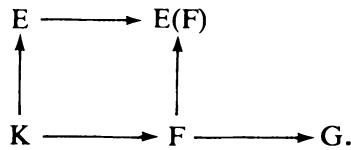
\includegraphics[keepaspectratio]{images/part001_e5f97af6.jpg}}\\
FIG. 2.

The condition is necessary: suppose that E and G are linearly disjoint over K. The same then holds of E and F (Prop. 7); on the other hand, if B is a basis of E over K, this is also a basis of the algebra F{[}E{]} over F; since B is by hypothesis free over G, F{[}E{]} and G are linearly disjoint over F, and the same is true of E(F) = F(E) and G, by Prop. 6.

The condition is sufficient: with the same notation it implies that B is free over F, hence it is a basis of F{[}E{]} over F; since F{[}E{]} and G are by hypothesis linearly disjoint over F, B is free over G, and this shows that E and G are linearly disjoint over K.

\section{ALGEBRAIC EXTENSIONS}

\subsection{Algebraic elements of an algebra}

Let \(\mathbf{A}\) be an algebra over a field \(\mathbf{K}\) and \(x\) an element of \(\mathbf{A}\) . Two cases are possible:

\begin{enumerate}
\def\labelenumi{\alph{enumi})}
\item
  The family of monomials \((x^{n})_{n\in\mathbb{N}}\) is free over K. Then we say that x is transcendental over K. There is an isomorphism of the polynomial algebra K{[}X{]} onto the subalgebra K{[}x{]} of A generated by x, and the latter is of infinite degree over K.
\item
  There exists an integer \(n \geqslant 1\) such that the monomials \(1, x, \ldots, x^{n-1}, x^n\) are linearly dependent; it comes to the same to say that there exists a polynomial \(f \neq 0\) in \(\mathbf{K}[\mathbf{X}]\) such that \(f(x) = 0\) . Then we say that \(x\) is algebraic over \(\mathbf{K}\) . The least integer \(n \geqslant 1\) satisfying the above property is called the degree of \(x\) over \(\mathbf{K}\) . If the degree of \(x\) over \(\mathbf{K}\) is \(n\) , then the monomials \(1, x, \ldots, x^{n-1}\) are linearly independent over \(\mathbf{K}\) and there exist elements \(a_0, a_1, \ldots, a_{n-1}\) of \(\mathbf{K}\) such that
\end{enumerate}

\[
x ^ {n} = a _ {0} + a _ {1} x + \dots + a _ {n - 1} x ^ {n - 1}.
\]

The polynomial \(f(\mathbf{X}) = \mathbf{X}^n - \sum_{k=0}^{n-1} a_k \mathbf{X}^k\) is the unique monic polynomial of degree

\(n\) in \(\mathbf{K}[\mathbf{X}]\) such that \(f(x) = 0\) ; it is called the minimal polynomial of \(x\) over \(\mathbf{K}\) .

THEOREM 1. --- Let A be an algebra over a field K, x an element of A algebraic over K, n the degree and f the minimal polynomial of x over K.

\begin{enumerate}
\def\labelenumi{\alph{enumi})}
\item
  For a polynomial \(g \in \mathbf{K}[\mathbf{X}]\) to satisfy \(g(x) = 0\) it is necessary and sufficient that \(g\) should be a multiple of \(f\) .
\item
  The mapping \(g \mapsto g(x)\) defines by passage to quotients an isomorphism of the quotient algebra \(\mathbf{K}[\mathbf{X}] / (f)\) onto the algebra \(\mathbf{K}[x]\) , and the elements 1, x, \ldots, \(x^{n-1}\) form a basis of \(\mathbf{K}[x]\) over \(\mathbf{K}\) . In particular, \([\mathbf{K}[x]: \mathbf{K}] = n\) .
\item
  Assume that A is an integral domain. Then K{[}x{]} is a field and f the unique monic irreducible polynomial in K{[}X{]} such that \(f(x) = 0\) .
\item
  For \(x\) to be invertible in \(\mathbf{A}\) it is necessary and sufficient that \(f(0) \neq 0\) ; then we have \(x^{-1} \in \mathbf{K}[x]\) .
\end{enumerate}

There exists a unique algebra homomorphism \(\varphi: \mathbf{K}[\mathbf{X}] \to \mathbf{A}\) such that \(\varphi(\mathbf{X}) = x\) ; we have \(\varphi(\mathbf{P}) = \mathbf{P}(x)\) for every \(\mathbf{P} \in \mathbf{K}[\mathbf{X}]\) and the image of \(\varphi\) equals \(\mathbf{K}[x]\) . Let \(\mathfrak{a}\) be the kernel of \(\varphi\) ; by construction, the minimal polynomial \(f\) of \(x\) over \(\mathbf{K}\) belongs to \(\mathfrak{a}\) and it is the monic polynomial of least degree in \(\mathfrak{a}\) . Therefore (IV, p.~11, Prop. 11) we have \(\mathfrak{a} = (f)\) , whence \(a\) ). Assertion \(b\) ) follows at once from \(a\) ) and the Cor. of Prop. 10 of IV, p.~11.

Suppose that A is an integral domain. The algebra K{[}x{]} is then an integral domain and of finite degree over K, hence it is a field (V, p.~10, Cor.). The ideal (f) of K{[}x{]} is thus maximal, that means that f is irreducible in K{[}X{]} (IV, p.~13). Finally, let g be a monic irreducible polynomial in K{[}X{]} such that \(g(x) = 0\) ; by a) it is a multiple of f, hence g = f, and this proves c).

It remains to prove \(d\) ). There exists a polynomial \(g \in \mathbf{K}[\mathbf{X}]\) of degree \(n - 1\) and an element \(a\) of \(\mathbf{K}\) such that \(f(\mathbf{X}) = \mathbf{X}g(\mathbf{X}) + a\) , whence \(f(0) = a\) . If \(a = 0\) , we have \(xg(x) = f(x) = 0\) , and \(g(x) \neq 0\) , so then \(x\) is not invertible in \(\mathbf{A}\) . If on the other hand \(a \neq 0\) , then we have \(x \cdot [-a^{-1}g(x)] = 1\) , so \(x\) is then invertible in \(\mathbf{A}\) and \(x^{-1} = -a^{-1}g(x)\) .

COROLLARY 1. --- Let A be an algebra over a field K. For an element x of A to be algebraic over K it is necessary and sufficient that the subalgebra \(K[x]\) of A generated by x should be of finite degree over K. In particular, if A is of finite degree over K, every element of A is algebraic over K.

COROLLARY 2. --- Let E be an extension of K, A an algebra over E and x an element of A algebraic over K. Then x is algebraic over E, the minimal polynomial of x over E divides the minimal polynomial of x over K and the degree of x over E is at most equal to the degree of x over K.

For let \(f\) be the minimal polynomial of \(x\) over \(\mathbf{K}\) ; we have \(f(x) = 0\) and \(f \in \operatorname{E}[\mathbf{X}]\) , hence \(x\) is algebraic over \(\mathbf{E}\) and \(f\) is a multiple of the minimal polynomial of \(x\) over \(\mathbf{E}\) (Th. 1, a)).

Remark. --- Let E be an extension of a field K and x an element of E which is root of a monic irreducible polynomial \(f \in K[X]\) . Th. 1, c) then shows that f is the minimal polynomial of x over K.

Examples. --- * 1) In the field of complex numbers C, the number i is algebraic of degree 2 over the prime field Q; for if \(f(\mathbf{X}) = \mathbf{X}^{2} + 1\) , then \(f(i) = 0\) , and \(x^{2} + 1 \neq 0\) for all \(x \in Q\) , hence \(i \notin Q\) . The field \(\mathbf{Q}(i)\) is thus an extension of degree 2 of Q; it consists of all numbers \(a + bi\) , where a, b are rational. Likewise i is algebraic of degree 2 over the field R of real numbers, and C is an extension of degree 2 of R.

\begin{enumerate}
\def\labelenumi{\arabic{enumi})}
\setcounter{enumi}{1}
\tightlist
\item
  Let K be a field and F the field \(\mathrm{K}(\mathrm{X})\) of rational functions in one indeterminate over K. Let E be the subfield \(\mathrm{K}(\mathrm{X}^{3})\) of F; we have \(\mathrm{F} = \mathrm{E}(\mathrm{X})\) and X is algebraic over E, since it is a root of the polynomial \(Y^{3} - X^{3}\) of the ring \(E[Y]\) ; this polynomial is irreducible in \(E[Y]\) , for in the contrary case it would have at least one factor of the first degree, and there would then exist two non-zero polynomials \(u(\mathrm{X})\) , \(v(\mathrm{X})\) of \(K[X]\) such that \((u(\mathrm{X}^{3}))^{3} = \mathrm{X}^{3}(v(\mathrm{X}^{3}))^{3}\) which is absurd, for if m and n are the degrees of u and v, this would imply \(9m = 9n + 3\) , or \(3m = 3n + 1\) . The field F is thus of degree 3 over E, and every element of F may be written in just one way as a linear combination \(f(\mathrm{X}^{3}) + \mathrm{X}g(\mathrm{X}^{3}) + \mathrm{X}^{2}h(\mathrm{X}^{3})\) , where f, g, h are three rational fractions of \(\mathrm{K}(\mathrm{X})\) .
\end{enumerate}

*3) In the field \(\mathbf{R}\) of real numbers it may be shown \(^1\) that the number \(\pi\) is transcendental over the prime field \(\mathbf{Q}\) . *

\subsection{Algebraic extensions}

DEFINITION 1. --- An extension E of a field K is said to be algebraic (over K) if every element of E is algebraic over K. An extension E of K which is not algebraic is called transcendental (over K).

PROPOSITION 1. --- For an extension E of K to be algebraic it is necessary and sufficient that every sub-K-algebra A of E should be a field.

The condition is necessary: if E is algebraic over K and \(x \neq 0\) is an element of a sub-K-algebra A of E, then \(x^{-1} \in K[x] \subset A\) by V, p.~16, Th. 1, d). Therefore A is a field.

The condition is sufficient: if it is satisfied and x is an element \(\neq 0\) in E, then the ring K{[}x{]} is a field, hence \(x^{-1} \in K[x]\) ; in other words, there exists a polynomial \(g \in K[X]\) such that \(x^{-1} = g(x)\) , or also \(xg(x) - 1 = 0\) ; this shows x to be algebraic over K, hence E is an algebraic extension of K.

PROPOSITION 2. --- If an extension E of K is of finite degree n, then it is algebraic and the degree over K of each element of E divides n.

For, given \(x \in \mathbb{E}\) , \([\mathbf{K}(x): \mathbf{K}]\) is finite and divides \(n(\mathbf{V}, p. 10, \text{Cor. } 1)\) and hence \(x\) is algebraic over \(\mathbf{K}(\mathbf{V}, p. 17, \text{Cor. } 1)\) .

* There exist algebraic extensions of infinite degree, for example the algebraic closure of a finite field (V, p.~24, Remark 4). *

THEOREM 2. --- Let E be a finitely generated extension of K, generated by the elements \(a_1, \ldots, a_m\) which are algebraic over K; then E is an extension of finite degree of K. If the degree of \(a_i\) over K ( \(a_1, a_2, \ldots, a_{i-1}\) ) is \(n_i\) (for \(1 \leq i \leq m\) ), then the degree of E over K is \(n_1 n_2 \ldots n_m\) and the elements \(a_1^{\nu_1} a_2^{\nu_2} \ldots a_m^{\nu_m}\) ( \(0 \leq \nu_i \leq n_i - 1\) ) form a basis of E over K.

The elements \(a_i^{\nu_i}\) ( \(0 \leqslant \nu_i \leqslant n_i - 1\) ) form a basis of \(K(a_1, a_2, \ldots, a_i)\) over \(K(a_1, a_2, \ldots, a_{i-1})\) by Th. 1, b) of V, p.~16; the theorem therefore follows by induction on \(m\) from Prop. 25 of II, p.~222.

COROLLARY 1. --- Let E be an extension of K and A a subset of E consisting of elements that are algebraic over K. Then K(A) is algebraic over K and we have K{[}A{]} = K(A).

For each \(x \in \mathrm{K}(\mathrm{A})\) belongs to a field \(\mathrm{K}(\mathrm{F})\) , where F is a finite subset of A (V, p.~11, Cor.) ; now \(\mathrm{K}(\mathrm{F})\) is algebraic over K and equal to \(\mathrm{K}[\mathrm{F}]\) by Th. 2, hence x is algebraic over K and \(\mathrm{K}(\mathrm{A}) = \mathrm{K}[\mathrm{A}]\) .

COROLLARY 2. --- Let L be an extension of K and E, F subextensions of L. If F is algebraic over K, the subring K{[}E, F{]} of L generated by E ∪ F is a field coinciding with E(F) and algebraic over E.

For each element of F, being algebraic over K, is also algebraic over E (V, p.~17, Cor. 2) hence \(E(F)\) is an algebraic extension of E, and we have \(E(F) = E[F]\) by Cor. 1.

Remarks. --- 1) With the notation of Th. 2, E = K{[}a₁, a₂, \ldots, aₘ{]} and hence E is isomorphic to a quotient K{[}X₁, X₂, \ldots, Xₘ{]}/α; since E is a field, α is a maximal ideal in K{[}X₁, \ldots, Xₘ{]}.

\begin{enumerate}
\def\labelenumi{\arabic{enumi})}
\setcounter{enumi}{1}
\tightlist
\item
  Let \(\mathbf{E}\) be an algebraic extension of \(\mathbf{K}\) , of infinite degree. By Th. 2 there exists an infinite sequence \((a_n)_{n \geq 1}\) of elements of \(\mathbf{E}\) such that \(a_n \notin \mathbf{K}(a_1, a_2, \ldots, a_{n-1})\) ; Th. 2 shows further that the degree of \(\mathbf{K}(a_1, a_2, \ldots, a_n)\) over \(\mathbf{K}\) takes arbitrarily large values. In other words, if E is an algebraic extension of K such that the degrees \([F:K]\) of the subextensions F of E of finite degree over K are bounded, then E is an extension of finite degree of K.
\end{enumerate}

\subsection{Transitivity of algebraic extensions. Fields that are relatively algebraically closed in an extension field}

PROPOSITION 3. --- Let E and F be two extension fields of a field K such that \(K \subset E \subset F\) . For F to be algebraic over K it is necessary and sufficient that E should be algebraic over K and F algebraic over E.

The condition is necessary, by V, p.~17, Cor. 2. Let us show that it is sufficient. Let x be any element of F; it is algebraic over E; let \(g \in E[X]\) be its minimal polynomial over E. If A is the (finite) set of coefficients of g, then \(g \in K(A)[X]\) , hence x is algebraic over \(K(A)\) and \(K(A \cup \{x\}) = K(A)(x)\) is of finite degree over \(K(A)\) . Now \(A \subset E\) and E is algebraic over K, hence \(K(A)\) is of finite degree over K, by Th. 2. Therefore (V, p.~10, Th. 1), \(K(A \cup \{x\})\) is of finite degree over K, which shows x to be algebraic over K (V, p.~18, Prop. 2).

DEFINITION 2. --- A subfield K of a field E is said to be relatively algebraically closed in E if every element of E which is algebraic over K, belongs to K.

It comes to the same to say that K is the only algebraic extension of K contained in E. Every field K is relatively algebraically closed in itself. In § 4 we shall study the fields which are relatively algebraically closed in each extension field.

PROPOSITION 4. --- Let E be an extension of a field K; the set L of elements of E which are algebraic over K forms a subextension of E which is relatively algebraically closed in E.

For the field \(\mathbf{K}(\mathbf{L})\) is algebraic over \(\mathbf{K}\) (Cor. 1 of Th. 2), hence \(\mathbf{K}(\mathbf{L}) \subset \mathbf{L}\) ; it follows that \(\mathbf{K}(\mathbf{L}) = \mathbf{L}\) and \(\mathbf{L}\) is a field. On the other hand, if \(x \in \mathbf{E}\) is algebraic over \(\mathbf{L}\) , it is so also over \(\mathbf{K}\) (Prop. 3) and hence belongs to \(\mathbf{L}\) .

The extension L of K consisting of all the elements of E that are algebraic over K is called the relative algebraic closure of K in E; it is the largest algebraic extension of K contained in E.

\section{ALGEBRAICALLY CLOSED EXTENSIONS}

\subsection{Algebraically closed fields}

PROPOSITION 1. --- Let K be a field ; then the following properties are equivalent :

(AC) Every non-constant polynomial of \(\mathbf{K}[\mathbf{X}]\) splits in \(\mathbf{K}[\mathbf{X}]\) into a product of polynomials of degree 1 (distinct or not).

(AC') Every non-constant polynomial of K{[}X{]} has at least one root in K.

(AC'') Every irreducible polynomial in K{[}X{]} is of degree 1.

(AC''') Every algebraic extension of K is of degree 1 (in other words, K is relatively algebraically closed in every extension field of K).

Let us first prove the equivalence of the properties (AC), (AC') and (AC''). Clearly (AC) implies (AC''). Since every non-constant polynomial of K{[}X{]} is divisible by an irreducible polynomial (IV, p.~13, Prop. 13) and every polynomial of degree 1 in K{[}X{]} clearly admits a root in K, we see that (AC'') implies (AC'). The condition (AC') implies by induction on n, that every polynomial of degree n in K{[}X{]} is a product of n polynomials of degree 1 (IV, p.~14, Prop. 1), hence (AC') implies (AC).

It remains to see that \((AC'')\) and \((AC''')\) are equivalent. If \((AC'')\) holds, every element of an extension field L of K which is algebraic over K is of degree 1 (V, p.~16, Th. 1), hence belongs to K, which establishes \((AC''')\) . Conversely, let f be an irreducible polynomial of degree \(n \geqslant 1\) in K{[}X{]}; the quotient algebra \(K[X]/(f)\) is of degree n over K and is a field, hence an algebraic extension of degree n of K (V, p.~18, Prop. 2). Now it is clear that \((AC''')\) implies \((AC'')\) .

DEFINITION 1. --- A field K is said to be algebraically closed if it possesses the (equivalent) properties (AC), (AC'), (AC''), (AC''').

* Example 1. --- The field \(\mathbf{C}\) of complex numbers is algebraically closed (Gen.~Top., VIII, p.~100). *

A field K which is relatively algebraically closed in an extension field E of K is not necessarily algebraically closed (in effect every field is relatively algebraically closed in itself, and there exist fields that are not algebraically closed, for example Q or \(F_{p}\) * or \(R_{*}\) ). However :

PROPOSITION 2. --- Let \(\Omega\) be an algebraically closed field and K a subfield of \(\Omega\) . Then the relative algebraic closure \(\bar{\mathbf{K}}\) of K in \(\Omega\) is an algebraically closed field.

Let \(f\) be a non-constant polynomial in \(\bar{\mathbf{K}}[\mathbf{X}] \subset \Omega[\mathbf{X}]\) . Since \(\Omega\) is algebraically closed, the polynomial \(f\) has at least one root in \(\Omega\) , and since this root is algebraic over \(\bar{\mathbf{K}}\) , it belongs to \(\bar{\mathbf{K}}\) (V, p.~19, Prop. 4). Therefore \(\bar{\mathbf{K}}\) satisfies (AC').

* Example 2. --- By Prop. 2 the set of all complex numbers that are algebraic over Q (often called briefly algebraic numbers) is an algebraically closed field. *

PROPOSITION 3. --- Every algebraically closed field is infinite.

Let \(\mathbf{K}\) be a finite field and put \(f(\mathbf{X}) = 1 + \prod_{a\in \mathbf{K}}(\mathbf{X} - a)\) . The polynomial

\(f \in K[X]\) is non-constant and \(f(a) = 1\) for each \(a \in K\) . So the field K does not satisfy (AC') and hence is not algebraically closed.

THEOREM 1 (Steinitz). --- Let K be a field, E an algebraic extension of K and \(\Omega\) an algebraically closed extension of K; then there exists a K-homomorphism of E into \(\Omega\) .

By V, p.~13, Scholium, there exists an extension field \(\Omega'\) of \(\Omega\) and a K-homomorphism \(u\) of E into \(\Omega'\) . Let \(x \in E\) ; since \(x\) is algebraic over K, \(u(x)\) is algebraic over \(u(\mathbf{K})\) and a fortiori over \(\Omega\) (V, p.~17, Cor. 2); since \(\Omega\) is algebraically closed, we thus have \(u(x) \in \Omega\) . It follows that \(u\) maps E into \(\Omega\) .

\subsection{Splitting extensions}

DEFINITION 2. --- Let K be a field and \((f_{i})_{i\in I}\) a family of non-constant polynomials in K{[}X{]}. By a splitting extension of \((f_{i})_{i\in I}\) we understand any extension E of K with the following properties:

\begin{enumerate}
\def\labelenumi{\alph{enumi})}
\item
  For each \(i \in \mathbf{I}\) , the polynomial \(f_i\) splits in \(\mathbf{E}[\mathbf{X}]\) into a product of polynomials of degree 1.
\item
  For each \(i \in I\) let \(\mathbf{R}_i\) be the set of roots of \(f_i\) in \(E\) , then \(E = K\left(\bigcup_{i \in I} \mathbf{R}_i\right)\) .
\end{enumerate}

Sometimes the term « splitting field » is used instead of « splitting extension ».

Remarks. --- 1) For each \(i \in I\) let \(c_i\) be a non-zero element of K and let \(f_i' = c_i f_i\) . Then it is clear that every splitting extension for the family \((f_i)_{i \in I}\) is also a splitting extension for the family \((f_i')_{i \in I}\) and conversely. In particular, in studying splitting extensions we may limit ourselves to the case of monic polynomials.

\begin{enumerate}
\def\labelenumi{\arabic{enumi})}
\setcounter{enumi}{1}
\tightlist
\item
  Suppose that I is finite and put \(f = \prod_{i \in I} f_i\) . Using the uniqueness of the
\end{enumerate}

decomposition of a polynomial into irreducible factors in E{[}X{]} (IV, p.~13, Prop. 13), we can easily show that a splitting extension for the polynomial f is a splitting extension for the family \((f_{i})_{i \in I}\) , and conversely. In other words, the case of a finite family may be reduced to the case of a single polynomial.

\begin{enumerate}
\def\labelenumi{\arabic{enumi})}
\setcounter{enumi}{2}
\tightlist
\item
  Let \(f \in K[X]\) be a polynomial of degree \(\geqslant 1\) and let E be a splitting extension of f.~If \(x_{1}, \ldots, x_{n}\) are the roots of f in E, we thus have \(\mathrm{E} = \mathrm{K}(x_{1}, \ldots, x_{n})\) and \([E : K]\) is finite (V, p.~18, Th. 2); but it may happen that E is distinct from the subfields \(\mathrm{K}(x_{1}), \ldots, \mathrm{K}(x_{n})\) generated by a single root; this can happen even when f is irreducible \(^{1}\) . We note however that when f is irreducible, the fields \(\mathrm{K}(x_{i})\) all have the same degree n over K, and whenever E is equal to one of them, we have \([E : K] = n\) and hence \(\mathrm{E} = \mathrm{K}(x_{1}) = \cdots = \mathrm{K}(x_{n})\) .
\end{enumerate}

PROPOSITION 4. --- Let K be a field and \((f_{i})_{i\in I}\) a family of non-constant polynomials in K{[}X{]}; then there exists a splitting extension for the family \((f_{i})_{i\in I}\) .

We may take the polynomials \(f_{i}\) to be monic (Remark 1). Let \(i \in I\) and let the degree of \(f_{i}\) be \(d_{i}\) . By IV, p.~73, Prop. 5 there exists a commutative algebra \(A_{i}\) over \(K\) , not reduced to 0, and elements \(\xi_{i,1}, \ldots, \xi_{i,d_{i}}\) of \(A_{i}\) such that:

\begin{enumerate}
\def\labelenumi{\alph{enumi})}
\item
  the algebra \(\mathbf{A}_i\) is generated by \((\xi_{i,1},\dots,\xi_{i,d_i})\) ;
\item
  we have \(f_{i}(\mathbf{X}) = \prod_{k=1}^{d_{i}} (\mathbf{X} - \xi_{i,k})\) in \(\mathbf{A}_i[\mathbf{X}]\) .
\end{enumerate}

Let A be the tensor product of the family of algebras \((\mathbf{A}_{i})_{i\in I}\) and let \(\varphi_{i}\) be the canonical homomorphism of \(A_{i}\) into A (III, p.~470). The algebra A is then commutative and not reduced to 0; by Krull's theorem (I, p.~104), there exists thus a maximal ideal a in A and \(E = A/a\) is an extension of the field K.

Denote by \(\psi\) the canonical homomorphism of A into E and put \(x_{i,k} = \psi (\varphi_i(\xi_{i,k}))\) for \(i\in I\) and \(1\leqslant k\leqslant d_i\) . Since the algebra A is generated by \(\cup \varphi_i(A_i)\) , the extension E is generated by the family \((x_{i,k})\) . Further, we have \(i\in I\)

\(f_{i}(\mathbf{X}) = \prod_{k=1}^{d_{i}} (\mathbf{X} - x_{i,k})\) in E{[}X{]}. Therefore E is a splitting extension of the family \((f_{i})_{i \in I}\) .

PROPOSITION 5. --- Let K be a field, \((f_i)_{i \in I}\) a family of non-constant polynomials in K{[}X{]}, E an extension of K, and F, F' subextensions of E which are each a splitting extension of \((f_i)_{i \in I}\) . Then F = F'.

Let \(\mathbf{R}_i\) be the set of roots of \(f_i\) in \(\mathbf{E}\) and \(\mathbf{R} = \bigcup_{i\in I}\mathbf{R}_i\) . Since \(f_i\) is a product of

polynomials of the first degree lying in F{[}X{]}, we have \(R_{i} \subset F\) . By Def. 2, we have \(F = K(R)\) ; in the same way we find that \(F' = K(R)\) .

COROLLARY. --- Let K be a field, \((f_{i})_{i\in I}\) a family of non-constant polynomials in K{[}X{]} and F, F' splitting extensions of \((f_{i})_{i\in I}\) . Then there exists a K-isomorphism of F onto F'.

This follows from Prop. 5 and V, p.~13, Cor. of Prop. 4.

\subsection{Algebraic closure of a field}

DEFINITION 3. --- Let K be a field. By an algebraic closure of K we understand any extension of K which is algebraic and algebraically closed.

Examples. --- * 1) The field C of complex numbers is an algebraic closure of the field R of real numbers (Gen.~Top., VIII, p.~100) *

\begin{enumerate}
\def\labelenumi{\arabic{enumi})}
\setcounter{enumi}{1}
\tightlist
\item
  Let K be a field and \(\Omega\) an algebraically closed extension of K. If \(\bar{K}\) is the relative algebraic closure of K in \(\Omega\) , then by V, p.~20, Prop. 2, \(\bar{K}\) is an algebraic closure of K. * In particular the field of all algebraic numbers (V, p.~20, Ex. 2) is an algebraic closure of the field Q of rational numbers. *
\end{enumerate}

PROPOSITION 6. --- Let \(\Omega\) be an extension of a field \(K\) . For \(\Omega\) to be an algebraic closure of \(K\) it is necessary and sufficient that it should be algebraic and that each non-constant polynomial in \(K[X]\) should split in \(\Omega[X]\) into a product of factors of degree 1.

The condition is necessary by (AC). Conversely, suppose that \(\Omega\) is algebraic over K and every non-constant polynomial over K{[}X{]} is a product in \(\Omega[\mathbf{X}]\) of factors of degree 1. Let \(\Omega'\) be an algebraic extension of \(\Omega\) and let \(x \in \Omega'\) . Since \(x\) is algebraic over \(\Omega\) and \(\Omega\) is algebraic over K, \(x\) is algebraic over K (V, p.~19, Prop. 3). Let \(f\) be the minimal polynomial of \(x\) over K. By hypothesis the polynomial \(f \in \mathbf{K}[\mathbf{X}]\) splits in \(\Omega[\mathbf{X}]\) into a product of factors of degree 1, whence \(x \in \Omega\) . Thus we have \(\Omega' = \Omega\) and \(\Omega\) is algebraically closed because it satisfies ( \(\mathrm{AC}'''\) ).

Remark 1. --- If \(\Omega\) is algebraic over \(K\) and if every non-constant polynomial of \(K[X]\) has a root in \(\Omega\) then \(\Omega\) is an algebraic closure of \(K\) (V, p.~156, Ex. 20).

PROPOSITION 7. --- Let \(\Omega\) be an algebraic extension of a field \(\mathbf{K}\) .

\begin{enumerate}
\def\labelenumi{\alph{enumi})}
\item
  If \(\Omega\) is algebraically closed, then every algebraic extension of \(\mathbf{K}\) is isomorphic to a subextension of \(\Omega\) .
\item
  Conversely suppose that every algebraic extension of finite degree of K is isomorphic to a subextension of \(\Omega\) ; then \(\Omega\) is algebraically closed.
\end{enumerate}

Assertion a) follows from Th. 1 (V, p.~20). Now assume the hypotheses of b) and consider a non-constant polynomial \(f \in K[X]\) . Let E be a splitting field of f (V, p.~21, Prop. 4); since E is algebraic of finite degree over K (V, p.~18, Th. 2), we may suppose that E is a subextension of \(\Omega\) . Then the polynomial f is a product of polynomials of degree 1 in \(\Omega[X]\) and Prop. 6 shows that \(\Omega\) is algebraically closed.

We can now prove the existence and uniqueness (up to isomorphism) of the algebraic closure of a field.

THEOREM 2 (Steinitz). --- Let K be a field ; then there exists an algebraic closure of K. If \(\Omega\) and \(\Omega'\) are two algebraic closures of K, there exists a K-isomorphism of \(\Omega\) onto \(\Omega'\) .

By Prop. 6 an algebraic closure of K is nothing other than a splitting extension for the set of all non-constant polynomials in K{[}X{]}. Th. 2 therefore follows from V, p.~21, Prop. 4 and V, p.~22, Cor.

COROLLARY. --- Let K and K' be two fields, Ω an algebraic closure of K and Ω' an algebraic closure of K'. For every isomorphism u of K onto K' there exists an isomorphism v of Ω onto Ω' extending u.

It is enough to apply Th. 2 to the algebraic closures \(\Omega\) and \((\Omega', u)\) of \(\mathbf{K}\) .

Remarks. --- 2) In the notation of the preceding Corollary there exist in general K-automorphisms of \(\Omega\) distinct from the identity. Hence there is in general no uniqueness about the isomorphism \(v\) of \(\Omega\) onto \(\Omega'\) extending the isomorphisms \(u\) of K onto K'. For similar reasons there is in general more than one isomorphism of a splitting extension E onto a splitting extension E' for the same family \((f_i)_{i \in I}\) of polynomials. We recall that by contrast, for the perfect closure we have uniqueness (V, p.~5).

\begin{enumerate}
\def\labelenumi{\arabic{enumi})}
\setcounter{enumi}{2}
\tightlist
\item
  Let K be a field and \(\Omega\) an algebraic closure of K. Then the following construction may be given for a splitting extension for a family \((f_{i})_{i\in I}\) of non-constant polynomials in K{[}X{]}: let \(R_{i}\) be the set of roots of \(f_{i}\) in \(\Omega\) and let \(R=\bigcup_{i\in I}R_{i}\) . Then \(K(R)\) is the unique subextension of \(\Omega\) which is a splitting
\end{enumerate}

extension for \((f_i)_{i\in I}\) (V, p.~22, Prop. 5).

\begin{enumerate}
\def\labelenumi{\arabic{enumi})}
\setcounter{enumi}{3}
\tightlist
\item
  Let K be a finite field and \(\Omega\) an algebraic closure of K. Then \(\Omega\) is infinite (V, p.~20, Prop. 3); since every extension of finite degree of K is a finite field, \(\Omega\) is an algebraic extension of infinite degree of K.
\end{enumerate}

\section{p-RADICAL EXTENSIONS}

Throughout this paragraph the letter p denotes an integer which is either 1 or a prime number. All the fields considered are of characteristic exponent p.~All the results stated in this paragraph are trivial when p = 1.

\subsection{p-radical elements}

DEFINITION 1. --- Let K be a field and E an extension of K. An element x of E is said to be p-radical over K if there exists an integer \(m \geqslant 0\) such that \(x^{p^{m}} \in K\) ; the least of these integers is called the height of x (over K).

PROPOSITION 1. --- Let E be an extension of a field K and x a p-radical element of height e over K; put \(a = x^{p^{e}}\) . Then \(a \in K\) and the minimal polynomial of x over K is \(X^{p^{e}} - a\) . Further we have \([\mathbf{K}(x): \mathbf{K}] = p^{e}\) .

It suffices to prove that the polynomial \(X^{p^{e}} - a\) is irreducible in K{[}X{]}. By the definition of height of x we have \(a \notin K^{p}\) , so that the proposition follows from the lemma :

Lemma 1. --- Let K be a field and a an element of K such that \(a \notin \mathbf{K}^p\) . Then for every integer \(e \geqslant 0\) , the polynomial \(f(\mathbf{X}) = \mathbf{X}^{p^e} - a\) is irreducible in \(\mathbf{K}[\mathbf{X}]\) .

Let \(\Omega\) be an algebraic closure of \(\mathbf{K}\) and let \(b\) be the element \(a^{p^{-e}}\) of \(\Omega\) ; we denote by \(g\) the minimal polynomial of \(b\) over \(\mathbf{K}\) . We have \(f(\mathbf{X}) = (\mathbf{X} - b)^{p^e}\) and hence every irreducible polynomial in \(\mathbf{K}[\mathbf{X}]\) which divides \(f\) admits \(b\) as root, and hence is equal to \(g\) . There exists thus (IV, p.~13, Prop. 13) an integer \(q \geqslant 1\) such that \(f = g^q\) ; since \(q\) divides the degree \(p^e\) of \(f\) , there exists an integer \(e'\) such that \(0 \leqslant e' \leqslant e\) and \(q = p^{e'}\) . If \(c\) is the constant term of \(g\) , we have \(-a = c^q\) ; since we assumed that \(a\) does not lie in \(\mathbf{K}^p\) , we must have \(q = 1\) , that is, \(f = g\) , so the lemma follows.

\subsection{\texorpdfstring{\(p\)-radical extensions}{p-radical extensions}}

DEFINITION 2. --- Let E be an extension of a field K. We shall say that E is p-radical \(^{1}\) (over K) if every element of E is p-radical over K. When this is so, E is said to be of finite height when the set of heights of elements of E is bounded above and we call the height of E the maximum of the heights of its elements.

We note that every \(p\) -radical extension of a perfect field (in particular of a field of characteristic 0) is trivial.

Let K be a field.. The p-radical extensions of height 0 of K are the trivial extensions. Every p-radical extension of K is algebraic. If E is a p-radical extension of K and F a p-radical extension of E, then F is a p-radical extension of K: for, given any \(x \in F\) , there exists an integer \(m \geqslant 0\) such that \(x^{p^{m}} \in E\) and an integer \(n \geqslant 0\) such that \((x^{p^{m}})^{p^{n}} \in \mathbf{K}\) , that is, \(x^{p^{m+n}} \in K\) .

PROPOSITION 2. --- Let E be an extension of a field K. For every integer \(n \geqslant 0\) let \(E_{n}\) be the set of elements of E which are p-radical of height \(\leqslant n\) over K, and let \(E_{\infty}\) be the set of all elements of E that are p-radical over K. Then \((\mathrm{E}_{n})_{n \geqslant 0}\) is an ascending sequence of subextensions of E whose union is \(E_{\infty}\) , and \(E_{\infty}\) is the largest p-radical extension of K contained in E.

For each integer \(n \geqslant 0\) the set \(E_{n}\) consists of all elements x of E such that \(x^{p^{n}} \in K\) ; since the mapping \(x \mapsto x^{p^{n}}\) is an endomorphism of the field E, we deduce that \(E_{n}\) is a subextension of E. The sequence \((\mathrm{E}_{n})_{n \geqslant 0}\) is ascending, with union \(E_{\infty}\) and hence \(E_{\infty}\) is a subextension of E (V, p.~11, Prop. 3). It is clear that \(E_{\infty}\) is a p-radical extension of K and that \(E_{\infty}\) contains every subextension of E which is p-radical over K.

COROLLARY. --- If an extension E of a field K is generated by a set of p-radical elements over K, then it is p-radical over K.

For \(E_{\infty}\) is a subextension of E and by hypothesis \(\mathrm{E} = \mathrm{K}(\mathrm{E}_{\infty})\) whence \(E = E_{\infty}\) ; so E is a p-radical extension of K.

Under the conditions of Proposition 2, \(E_{\infty}\) is said to be the relative p-radical closure of K in E.

We shall apply Prop. 2 particularly to the case where E is an algebraically closed extension of K; then E is perfect and we have \(E_{n} = K^{p^{-n}}\) for all \(n \geqslant 0\) . In this case we denote by \(K^{p^{-\infty}}\) the set of elements of E that are p-radical over K; it is the subfield of E which is the union of the ascending sequence \((\mathbf{K}^{p^{-n}})_{n \geqslant 0}\) of subfields of E. By Prop. 2, \(K^{p^{-\infty}}\) is the largest subextension of E which is p-radical over K; by Prop. 3 of V, p.~6, \(K^{p^{-\infty}}\) is a perfect closure of K and it is also the smallest perfect subfield of E containing K. When K is perfect we clearly have \(K = K^{p^{-n}} = K^{p^{-\infty}}\) for all n.~If K is imperfect, we have \(K \neq K^{p}\) , whence

\[
\mathbf {K} ^ {p ^ {- n}} \neq (\mathbf {K} ^ {p}) ^ {p ^ {- n}} = \mathbf {K} ^ {p ^ {- (n - 1)}}
\]

for \(n \geqslant 1\) ; the subfields \(\mathbf{K}^{p^{-n}}\) of \(E\) are then pairwise distinct and \(\mathbf{K}^{p^{-\infty}}\) is an algebraic extension of infinite degree of \(K\) .

PROPOSITION 3. --- Let K be a field, E an extension field of K which is p-radical over K and u a homomorphism of K into a perfect field F. Then there exists a unique homomorphism v of E into F extending u.

Let \(E_n\) be the set of elements of \(E\) which are \(p\) -radical of height \(\leqslant n\) over \(K\) . By Prop. 2 the field \(E\) is the union of the ascending sequence \((E_n)_{n \geqslant 0}\) of subfields. Let \(v\) be a homomorphism of \(E\) into \(F\) extending \(u\) ; for any \(x \in E_n\) we have \(x^{p^n} \in K\) , whence \(v(x)^{p^n} = v(x^{p^n}) = u(x^{p^n})\) ; we thus have \(v(x) = u(x^{p^n})^{p^{-n}}\) for all \(n \geqslant 0\) and all \(x \in E_n\) , whence the uniqueness of the extension of \(u\) to \(E\) .

Let \(n\) be a positive integer; for any \(x \in \mathrm{E}_n\) we have \(x^{p^n} \in \mathbf{K}\) and since \(F\) is perfect, we can define an element \(v_n(x)\) of \(F\) by \(v_n(x) = u(x^{p^n})^{p^{-n}}\) . It is clear that \(v_n\) is a homomorphism of \(E_n\) into \(F\) , that \(v_0 = u\) and that \(v_{n+1}\) induces \(v_n\) on \(E_n\) . Hence there exists a homomorphism \(v\) of \(E\) into \(F\) inducing \(v_n\) on \(E_n\) for all \(n \geqslant 0\) and, in particular, coinciding with \(v_0 = u\) on \(E_0 = K\) .

COROLLARY. --- For an extension E of a field K to be a perfect closure of K it is necessary and sufficient that it should be a p-radical extension of K and that the field E should be perfect.

The Corollary is trivial when p = 1; suppose then that \(p \neq 1\) . The stated conditions are necessary by V, p.~5, Th. 3; they are sufficient by Prop. 3.

PROPOSITION 4. --- Let E be a p-radical extension of finite degree of a field K. Then {[}E : K{]} is a power of the characteristic exponent p of K.

Since E is a p-radical extension of finite degree of K, there are elements \(a_{1}, \ldots, a_{m}\) of E, p-radical over K, such that \(\mathrm{E} = \mathrm{K}(a_{1}, \ldots, a_{m})\) . Let i be in the range 1 to m; since \(a_{i}\) is a fortiori p-radical over \(\mathrm{K}(a_{1}, \ldots, a_{i-1})\) , the degree

\[
n _ {i} = \left[ \mathrm{K} (a _ {1}, \dots , a _ {i}): \mathrm{K} (a _ {1}, \dots , a _ {i - 1}) \right]
\]

is a power of \(p\) (V, p.~24, Prop. 1). We have \([\mathrm{E}:\mathbf{K}] = n_1\ldots n_m\) by V, p.~18, Th. 2, whence the result.

\section{ETALE ALGEBRAS}

Throughout this paragraph K denotes a field.

\subsection{Linear independence of homomorphisms}

Let L be an extension of K and V a vector space over K. In this paragraph we shall denote by \(\operatorname{Hom}_{\mathbf{K}}(\mathbf{V},\mathbf{L})\) the set of all K-linear mappings of V into L, equipped with the vector space structure on L such that :

\[
(f + g) (x) = f (x) + g (x), \quad (\alpha f) (x) = \alpha f (x)\tag{1}
\]

for \(x \in \mathbf{V}\) , \(\alpha \in \mathbf{L}\) and \(f, g\) in \(\operatorname{Hom}_{\mathbf{K}}(\mathbf{V}, \mathbf{L})\) . Let \(\mathbf{V}_{(\mathbf{L})} = \mathbf{L} \otimes_{\mathbf{K}} \mathbf{V}\) be the vector space on \(\mathbf{L}\) derived from \(\mathbf{V}\) by extension of scalars, and \((\mathbf{V}_{(\mathbf{L})})^*\) its dual. By II, p.~277 we have a canonical isomorphism \(u \mapsto \tilde{u}\) of vector \(\mathbf{L}\) -spaces from \((\mathbf{V}_{(\mathbf{L})})^*\) onto \(\operatorname{Hom}_{\mathbf{K}}(\mathbf{V}, \mathbf{L})\) such that \(\tilde{u}(x) = u(1 \otimes x)\) for \(x \in \mathbf{V}\) and \(u\) in \((\mathbf{V}_{(\mathbf{L})})^*\) . If \(\mathbf{V}\) is of finite dimension \(n\) over \(\mathbf{K}\) , the vector space \((\mathbf{V}_{(\mathbf{L})})\) over \(\mathbf{L}\) is of dimension \(n\) , as well as its dual \((\mathbf{V}_{(\mathbf{L})})^* = \mathbf{V}_{(\mathbf{L})}^*\) , whence the formula

\[
[ \operatorname{Hom} _ {K} (V, L): L ] = [ V: K ].\tag{2}
\]

THEOREM 1. --- Let L be an extension of a field K and A an algebra over K ; let H be the set of all K-algebra homomorphisms of A into L. Then H is a free subset of the vector space \(\operatorname{Hom}_{K}(A, L)\) over L.

Let us show by induction on the integer \(n \geqslant 0\) that every sequence \((u_1, \ldots, u_n)\) of distinct elements of \(\mathcal{H}\) is free. The case \(n = 0\) being trivial, we may henceforth suppose that \(n \geqslant 1\) ; let \(\alpha_1, \ldots, \alpha_n\) be elements of \(L\) such that \(\sum_{i=1}^{n} \alpha_i u_i = 0\) . For \(x, y\) in \(A\) we have

\[
\sum_ {i = 1} ^ {n - 1} \alpha_ {i} [ u _ {i} (x) - u _ {n} (x) ] \cdot u _ {i} (y) = \sum_ {i = 1} ^ {n} \alpha_ {i} u _ {i} (x y) - u _ {n} (x) \sum_ {i = 1} ^ {n} \alpha_ {i} u _ {i} (y) = 0,
\]

whence \(\sum_{i=1}^{n-1} \alpha_i [u_i(x) - u_n(x)] \cdot u_i = 0\) . By the induction hypothesis, the elements

\(u_{1}, \ldots, u_{n-1}\) of \(\mathscr{H}\) are linearly independent, whence \(\alpha_{i}[u_{i}(x) - u_{n}(x)] = 0\) for \(1 \leqslant i \leqslant n-1\) and for all x in A. Since the \(u_{i}\) are distinct, this implies that \(\alpha_{i} = 0\) for \(i \neq n\) , hence \(\alpha_{n}u_{n} = 0\) and so \(\alpha_{n} = \alpha_{n}u_{n}(1) = 0\) (on denoting by 1 the unit element of A). We have thus shown that \(\alpha_{1}, \ldots, \alpha_{n-1}, \alpha_{n}\) are zero, and this proves the theorem.

COROLLARY 1. --- Let \(\Gamma\) be a monoid, L a field and X a set of homomorphisms of \(\Gamma\) into the multiplicative monoid of L. Then X is a free subset of the vector L-space \(L^{\Gamma}\) of mappings of \(\Gamma\) into L.

Let A be the algebra of the monoid \(\Gamma\) with coefficients in L and \((e_{\gamma})_{\gamma \in \Gamma}\) the canonical basis of A over L (III, p.~446). For every L-linear mapping \(u\) of A into L let us write \(\tilde{u}(\gamma) = u(e_{\gamma})\) (for \(\gamma \in \Gamma\) ); then the mapping \(u \mapsto \tilde{u}\) is an isomorphism of vector L-spaces of \(\operatorname{Hom}_{L}(A, L)\) onto \(L^{\Gamma}\) which maps onto X the set of L-algebra homomorphisms of A into L. Now it suffices to apply Th. 1 with \(K = L\) .

COROLLARY 2 (Dedekind's theorem). --- Let E and L be two extensions of K. The set of K-homomorphisms of E into L is free over L. If E is of finite degree over K, the number of K-homomorphisms of E into L is at most equal to {[}E:K{]}.

The last assertion follows from the first, taking account of Formula (2).

\subsection{Algebraic independence of homomorphisms}

THEOREM 2. --- Let K be an infinite field, L an extension of K and A an algebra over K. Let \(u_1, \ldots, u_n\) be distinct K-algebra homomorphisms of A into L and f a polynomial in L{[}X₁, \ldots, Xₙ{]}. If we have \(f(u_1(x), \ldots, u_n(x)) = 0\) for all \(x \in \mathbf{A}\) , then \(f = 0\) .

Let B be the set of elements of \(L^{n}\) of the form \((u_{1}(x), \ldots, u_{n}(x))\) with \(x \in A\) . By Th. 1, there is no sequence \((\alpha_{1}, \ldots, \alpha_{n})\) of elements not all zero in L such that \(\sum_{i=1}^{n} \alpha_{i} u_{i}(x) = 0\) for all \(x \in A\) ; therefore (II, p.~301, Th. 7) B generates

the vector space \(\mathbf{L}^n\) over \(\mathbf{L}\) . So there exist elements \(a_1, \ldots, a_n\) of \(\mathbf{A}\) such that the matrix \((u_i(a_j))_{1 \leqslant i, j \leqslant n}\) is invertible.

Let us define the polynomial \(g \in L[Y_1, \ldots, Y_n]\) by

\[
g \left(\mathrm{Y} _ {1}, \dots , \mathrm{Y} _ {n}\right) = f \left(\sum_ {j = 1} ^ {n} u _ {1} \left(a _ {j}\right) \mathrm{Y} _ {j}, \dots , \sum_ {j = 1} ^ {n} u _ {n} \left(a _ {j}\right) \mathrm{Y} _ {j}\right).\tag{3}
\]

Let \(y_{1}, \ldots, y_{n}\) be in K; writing \(x = \sum_{i=1}^{n} y_{i} a_{i}\) , we have

\[
g \left(y _ {1}, \dots , y _ {n}\right) = f \left(u _ {1} (x), \dots , u _ {n} (x)\right), \quad \text { whence } \quad g \left(y _ {1}, \dots , y _ {n}\right) = 0
\]

by the hypothesis on \(f\) . Since the field \(K\) is infinite, we have \(g = 0\) (IV, p.~18, Cor. 2); now the matrix \((u_i(a_j))\) has an inverse \((b_{ij})\) and we have

\[
f \left(\mathrm{X} _ {1}, \dots , \mathrm{X} _ {n}\right) = g \left(\sum_ {j = 1} ^ {n} b _ {1 j} \mathrm{X} _ {j}, \dots , \sum_ {j = 1} ^ {n} b _ {n j} \mathrm{X} _ {j}\right),\tag{4}
\]

whence \(f = 0\) .

Th. 2 has no analogue for finite fields. Thus let K be a finite field with q elements, A = L = K and \(f(X) = X^{q} - X\) . We have \(x^{q} = x\) for all \(x \in K\) (V, p.~93, Prop. 2); therefore if u is the identity automorphism of K, we have \(f(u(x)) = 0\) for all \(x \in K\) , even though f is not zero.

\subsection{Diagonalizable algebras and etale algebras}

DEFINITION 1. --- Let A be an algebra over K; then A is said to be diagonalizable if there exists an integer \(n \geqslant 0\) such that A is isomorphic to the product algebra \(\mathbf{K}^n\) . We say that A is diagonalized by an extension L of K if the algebra \(\mathbf{A}_{(L)}\) over L derived from A by extension of scalars is diagonalizable. We shall say that A is etale if there exists an extension of K which diagonalizes A.

We recall that the product algebra \(K^{n}\) is the vector space \(K^{n}\) equipped with the product defined by

\[
\left(x _ {1}, \dots , x _ {n}\right) \cdot \left(y _ {1}, \dots , y _ {n}\right) = \left(x _ {1} y _ {1}, \dots , x _ {n} y _ {n}\right).\tag{5}
\]

If \(\varepsilon_1, \ldots, \varepsilon_n\) is the canonical basis of \(\mathbf{K}^n\) , we have

\[
\varepsilon_ {i} ^ {2} = \varepsilon_ {i}, \quad \varepsilon_ {i} \varepsilon_ {j} = 0 \quad \text { if } \quad i \neq j\tag{6}
\]

and \(1 = \varepsilon_{1} + \dots +\varepsilon_{n}\)

Every etale algebra over K is commutative and of finite degree over K.

PROPOSITION 1. --- Let A be an algebra of finite degree n over the field K ; then the following conditions are equivalent :

\begin{enumerate}
\def\labelenumi{\alph{enumi})}
\item
  The algebra \(\mathbf{A}\) is diagonalizable.
\item
  There is a basis \((e_1, \ldots, e_n)\) of A such that \(e_i^2 = e_i\) and \(e_i e_j = 0\) for \(i \neq j\) .
\item
  The K-algebra homomorphisms of A into K generate the dual of the vector K-space A.
\item
  Every A-module is a direct sum of submodules which are of dimension 1 over K.
\end{enumerate}

The equivalence of \(a)\) and \(b)\) follows from Formula (6); on the other hand the \(n\) projections \(\mathbf{K}^n \to \mathbf{K}\) are algebra homomorphisms, hence \(a)\) implies \(c)\) . If \(c)\) holds, the algebra homomorphisms of \(\mathbf{A}\) into \(\mathbf{K}\) form a basis of the dual of \(\mathbf{A}\) (V, p.~27, Th. 1), we denote them by \(u_1, \ldots, u_n\) ; then \(a \mapsto (u_i(a))\) is an isomorphism of \(\mathbf{A}\) onto the algebra \(\mathbf{K}^n\) , whence \(a)\) . We have thus established the equivalence of the conditions \(a), b)\) and \(c)\) .

Suppose that \(b)\) holds and let \(\mathbf{M}\) be an A-module; then the homotheties \((e_i)_{\mathbf{M}}\) of ratio \(e_i\) are projectors of \(\mathbf{M}\) , and \(\mathbf{M}\) is a direct sum of the \(e_i\mathbf{M}\) , which are sub-A-modules. We may thus suppose that there exists an index \(i\) such that \((e_j)_{\mathbf{M}} = 0\) for \(j \neq i\) . Hence every vector subspace of \(\mathbf{M}\) is a sub-A-module, whence \(d)\) .

Conversely suppose that \(d\) holds and consider the A-module \(\mathbf{A}_{s}\) . There exists then a basis \((f_{i})\) of the vector K-space \(\mathbf{A}\) such that \(\mathbf{A}f_{i} = \mathbf{K}f_{i}\) for \(i = 1, \ldots, n\) . After replacing each \(f_{i}\) by a suitable scalar multiple, if necessary, we may suppose that \(1 = f_{i} + \cdots + f_{n}\) . If \(i \neq j\) , then \(f_{i}f_{j}\) belongs to \(\mathbf{A}f_{i} \cap \mathbf{A}f_{j} = \mathbf{K}f_{i} \cap \mathbf{K}f_{j}\) hence it is zero. Now \(f_{i} = f_{i}f_{1} + \cdots + f_{i}f_{n} = f_{i}^{2}\) , whence \(b\) ).

COROLLARY. --- Let L be an extension of K and H the set of algebra homomorphisms of A into L. We have Card \(H \leq [A:K]\) , with equality if and only if A is diagonalized by L. If A is diagonalized by L, then H is a basis of the vector L-space \(\operatorname{Hom}_{\mathbf{K}}(\mathbf{A},\mathbf{L})\) .

The vector space \(\operatorname{Hom}_{\mathbf{K}}(\mathbf{A},\mathbf{L})\) over L has dimension \([A:K]\) , by Formula (2), and H is a free subset of \(\operatorname{Hom}_{\mathbf{K}}(\mathbf{A},\mathbf{L})\) by Th. 1 (V, p.~27). We thus have Card \(H \leqslant [A:K]\) with equality if and only if H is a basis of \(\operatorname{Hom}_{\mathbf{K}}(\mathbf{A},\mathbf{L})\) . There exists an isomorphism of vector L-spaces, say \(\pi: \operatorname{Hom}_{\mathbf{K}}(\mathbf{A}, \mathbf{L}) \to \mathbf{A}_{(\mathbf{L})}^{*}\) , characterized by \(u(x) = (\pi u)(1 \otimes x)\) for \(x \in \mathbf{A}\) , and \(\pi\) maps \(\mathcal{H}\) onto the set \(\mathcal{H}_{\mathbf{L}}\) of L-algebra homomorphisms of \(\mathbf{A}_{(\mathbf{L})}\) into L. Finally the equivalence of \(a)\) and \(c)\) in Prop. 1 shows that the algebra \(\mathbf{A}_{(\mathbf{L})}\) over L is diagonalizable if and only if \(\mathcal{H}_{\mathbf{L}}\) generates the vector space \(\mathbf{A}_{(\mathbf{L})}^{*}\) over L. This completes the proof of the Corollary.

PROPOSITION 2. --- Let A be an algebra over K and \(\Omega\) an algebraically closed extension of K. The following assertions are equivalent:

\begin{enumerate}
\def\labelenumi{\alph{enumi})}
\item
  The algebra \(\mathbf{A}\) is etale.
\item
  There exists an extension of finite degree which diagonalizes A.
\item
  The extension \(\Omega\) of \(\mathbf{K}\) diagonalizes \(\mathbf{A}\) .
\end{enumerate}

Suppose that A is etale. Let n be the degree of A over K, let L be an extension of K which diagonalizes A and let H be the set of algebra homomorphisms of A into L. By the Cor. to Prop. 1 we have Card H = n.~On the other hand, for each \(u \in H\) , we have \([u(A):K] \leqslant n\) . By V, p.~18, Th. 2, the subextension \(L'\) of L generated by the images of elements of H is of finite degree over K. Since there exist n distinct homomorphisms of A into \(L'\) , the extension \(L'\) diagonalizes A, by the Cor. 1 of Prop. 1. This shows that a) implies b).

Since every extension of finite degree of K is isomorphic to a subextension of \(\Omega\) (V, p.~20, Th. 1), b) implies c). Finally c) clearly implies a).

\subsection{Subalgebras of an etale algebra}

PROPOSITION 3. --- Let A be an etale algebra over K. There exist only a finite number of subalgebras and ideals of A. Moreover, every extension of K which diagonalizes A also diagonalizes every subalgebra and every quotient algebra of A; in particular these algebras are etale.

It suffices to show that an algebra \(K^{n}\) has only a finite number of subalgebras and ideals, and that the subalgebras and quotient algebras of \(K^{n}\) are diagonalizable. We denote by \((\varepsilon_{1},\ldots,\varepsilon_{n})\) the canonical basis of \(K^{n}\) .

Let A be a subalgebra of \(K^{n}\) and let \(v_{1}, \ldots, v_{n}\) be the restrictions to A of the n projections \(K^{n} \rightarrow K\) . Since the intersection of the kernels of the \(v_{i}\) is clearly 0, the \(v_{i}\) generate the vector K-space dual to A (II, p.~302, Cor. 1); hence the K-algebra A is diagonalizable (V, p.~29, Prop. 1).

For every subset I of \(\{1, 2, \ldots, n\}\) put \(\varepsilon_{I} = \sum_{i \in I} \varepsilon_{i}\) . It is clear that the elements

\(\varepsilon_{I}\) are idempotents of \(K^{n}\) ; we have \(\varepsilon_{I}=0\) if and only if I is empty, and \(\varepsilon_{I}\varepsilon_{J}=\varepsilon_{I\cap J}\) . By what has been said, every subalgebra A of \(K^{n}\) is diagonalizable; by condition b) of Prop. 1 every subalgebra A of \(K^{n}\) therefore admits a basis \((\varepsilon_{I_{1}},\ldots,\varepsilon_{I_{p}})\) , where \((I_{1},\ldots,I_{p})\) is a partition of \(\{1,2,\ldots,n\}\) , and there are only a finite number of such subalgebras.

For every subset I of \(\{1,2,\ldots,n\}\) let \(a_{I}\) be the vector subspace of \(K^{n}\) having as basis the idempotents \(\varepsilon_{i}\) for \(i\in I\) ; then it is clear that \(a_{I}\) is an ideal of \(K^{n}\) ; moreover if \(J=\{1,2,\ldots,n\}-I\) , then the residue classes \(\overline{\varepsilon}_{j}\) of \(\varepsilon_{j} \mod a_{I}\) for \(j\in J\) form a basis of \(K^{n}/a_{I}\) . We have \(\overline{\varepsilon}_{j}^{2}=\overline{\varepsilon}_{j}\) and \(\overline{\varepsilon}_{j}\overline{\varepsilon}_{k}=0\) if \(j\neq k\) , hence the algebra \(K^{n}/a_{I}\) is diagonalizable, by Prop. 1 of V, p.~29.

It remains to show that every ideal of \(K^{n}\) is of the form \(a_{I}\) . Let I be the set of integers i such that \(1 \leqslant i \leqslant n\) and \(\varepsilon_{i} \in a\) , then \(a_{I} \subset a\) . Let \(x = x_{1}\varepsilon_{1} + \cdots + x_{n}\varepsilon_{n}\) be an element of a (with \(x_{1}, \ldots, x_{n}\) in K) and let i be in \(\{1, 2, \ldots, n\} - I\) . We have \(x_{i}\varepsilon_{i} = x\varepsilon_{i} \in a\) , and \(\varepsilon_{i} \notin a\) , whence \(x_{i} = 0\) . Thus \(x = \sum_{i \in I} x_{i}\varepsilon_{i}\) and this shows that

\(x \in a_{1}\) . We have now shown \(a \subset a_{1}\) , whence finally \(a = a_{1}\) .

COROLLARY. --- Let \(A_{1}, \ldots, A_{m}\) be algebras over K and \(A = A_{1} \times \cdots \times A_{m}\) . For A to be etale it is necessary and sufficient that \(A_{1}, \ldots, A_{m}\) are etale.

Suppose that A is etale; each of the algebras \(A_{1}, \ldots, A_{m}\) is isomorphic to a quotient of A, and hence is etale by Prop. 3. Conversely, every extension of K which diagonalizes \(A_{1}, \ldots, A_{m}\) clearly diagonalizes A.

\subsection{Separable degree of a commutative algebra}

Let A be a commutative algebra of finite degree n over K. For any extension L of K, the number \(h(L)\) of algebra homomorphisms of A into L is finite and is bounded above by n (V, p.~29, Cor.).

Lemma 1. --- Let \(\Omega\) be an algebraic closure of K; then we have \(h(L) \leqslant h(\Omega)\) for every extension L of K, with equality when L is algebraically closed.

Let \(L'\) be the algebraic closure of K in L. For every homomorphism u of A into L we have \([u(A):K] \leqslant n\) , hence \(u(A) \subset L'\) by V, p.~18, Prop. 2; we thus have \(h(L') = h(L)\) . Since the extension \(L'\) of K is isomorphic to a subextension of \(\Omega(V, p. 20, Th. 1)\) , we have \(h(L') \leqslant h(\Omega)\) . If L is algebraically closed, then \(L'\) is an algebraic closure of K; the extensions \(L'\) and \(\Omega\) of K are then isomorphic (V, p.~23, Th. 2) and so \(h(L') = h(\Omega)\) ; the Lemma follows directly from this.

By Lemma 1, the number \(h(\mathbf{L})\) has the same value for all algebraically closed extensions \(\mathbf{L}\) of \(\mathbf{K}\) ; this number will be denoted by \([\mathbf{A}:\mathbf{K}]_s\) and called the separable degree of \(\mathbf{A}\) .

Let \(\mathbf{A}\) and \(\mathbf{B}\) be two commutative algebras of finite degree over \(\mathbf{K}\) . We shall establish the formula

\[
[ \mathbf {A} \otimes_ {\mathbf {K}} \mathbf {B}: \mathbf {K} ] _ {s} = [ \mathbf {A}: \mathbf {K} ] _ {s}. [ \mathbf {B}: \mathbf {K} ] _ {s}.\tag{7}
\]

Let \(L\) be an algebraically closed extension of \(K\) and denote by \(\mathcal{H}(A)\) the set of algebra homomorphisms of \(A\) into \(L\) , and similarly define \(\mathcal{H}(B)\) and \(\mathcal{H}(A \otimes_K B)\) . By definition we have Card \(\mathcal{H}(A) = [A : K]_s\) and corresponding formulae for \([B:K]_{s}\) and \([A\otimes_{K}B:K]_{s}\) . Moreover (III, p.~465, Formula (6)), the formula \((u*v)(a\otimes b)=u(a)v(b)\) defines a bijection \((u,v)\mapsto u*v\) of \(\mathcal{H}(A)\times\mathcal{H}(B)\) onto \(\mathcal{H}(A\otimes_{K}B)\) , whence Formula (7) follows.

Let \(\mathbf{K}'\) be an extension of \(\mathbf{K}\) ; we shall prove the formula

\[
[ \mathbf {A} _ {(\mathbf {K} ^ {\prime})}: \mathbf {K} ^ {\prime} ] _ {s} = [ \mathbf {A}: \mathbf {K} ] _ {s}.\tag{8}
\]

For take L to be an algebraic closure of \(K'\) . The formula \(\tilde{u}(x)=u(1\otimes x)\) (for \(x\in A\) ) defines a bijection \(u\mapsto\tilde{u}\) between the set of \(K'\) -homomorphisms of \(\mathrm{A}_{(\mathrm{K}')}\) into L and the set of K-homomorphisms of A into L, whence (8).

Finally, suppose that \(K'\) is an extension of finite degree of K; if \(A'\) is a commutative \(K'\) -algebra of finite degree, then it is also a commutative K-algebra of finite degree and we have \([A':K] = [A':K']\) . \([K':K]\) (V. p.~10, Th. 1). We shall prove the formula

\[
[ \mathrm{A} ^ {\prime}: \mathrm{K} ] _ {s} = [ \mathrm{A} ^ {\prime}: \mathrm{K} ^ {\prime} ] _ {s} \cdot [ \mathrm{K} ^ {\prime}: \mathrm{K} ] _ {s}.\tag{9}
\]

For let S (resp. T) be the set of K-homomorphisms of \(K'\) (resp. \(A'\) ) into an algebraic closure L of K; for every \(\sigma \in S\) we denote by \(T_{\sigma}\) the set of elements f of T such that \(f(\alpha, 1) = \sigma(\alpha)\) for all \(\alpha \in K'\) . Then the family \((\mathrm{T}_{\sigma})_{\sigma \in S}\) is a partition of T and we have Card \(S = [K': K]_{s}\) ; now for each \(\sigma \in S\) the set \(T_{\sigma}\) consists of \(K'\) -homomorphisms of \(A'\) into the algebraically closed extension \((L, \sigma)\) of \(K'\) , hence Card \(T_{\sigma} = [A': K']_{s}\) , and so we have proved (9).

PROPOSITION 4. --- Let A be a commutative algebra of finite degree over K; then \([A:K]_{s} \leqslant [A:K]\) with equality if and only if A is etale.

Let \(\Omega\) be an algebraic closure of K and \(\mathcal{H}\) the set of algebra homomorphisms of A into \(\Omega\) . We have Card \(\mathcal{H} = [\mathrm{A}:\mathrm{K}]_s\) , and A is etale if and only if A is diagonalized by the extension \(\Omega\) of K (V, p.~30, Prop. 2). Thus Prop. 4 follows from the Cor. of V, p.~29.

COROLLARY 1. --- Let A, B be two commutative algebras over K, of finite non-zero degrees. Then for the algebra \(C = A \otimes_{K} B\) to be etale it is necessary and sufficient for A and B to be etale.

We have \([C:K]=[A:K]\) . \([B:K]\) and the corresponding Formula (7) for the separable degrees. Further we have \([A:K]_{s}\leqslant[A:K]\) and corresponding formulae for B and C. It follows that \([C:K]=[C:K]_{s}\) if and only if we have both \([A:K]=[A:K]_{s}\) and \([B:K]=[B:K]_{s}\) ; now it is enough to apply Prop. 4.

COROLLARY 2. --- Let K' be an extension of K.

\begin{enumerate}
\def\labelenumi{\alph{enumi})}
\item
  For a K-algebra A to be etale, it is necessary and sufficient that the \(\mathbf{K}'\) -algebra \(\mathbf{A}_{(\mathbf{K}')}\) should be etale.
\item
  Let \(\mathbf{A}'\) be an algebra over \(\mathbf{K}'\) , not reduced to 0. For \(\mathbf{A}'\) to be etale over \(\mathbf{K}\) it is necessary and sufficient that \(\mathbf{A}'\) should be etale over \(\mathbf{K}'\) and \(\mathbf{K}'\) etale over \(\mathbf{K}\) .
\end{enumerate}

We argue as for Cor. 1, applying this time (8) for \(a\) and (9) for \(b\) .

\subsection{Differential characterization of etale algebras}

THEOREM 3. --- Let A be a commutative algebra of finite degree over K. For A to be etale it is necessary and sufficient that the module \(\Omega_{\mathrm{K}}(\mathrm{A})\) of K-differentials of A should be reduced to 0.

\begin{enumerate}
\def\labelenumi{\Alph{enumi})}
\item
  Let L be an algebraic closure of K (V, p.~23, Th. 2). For A to be etale it is necessary and sufficient that the algebra \(\mathbf{A}_{(L)}\) over L should be diagonalizable (V, p.~30, Prop. 2). Further, the A-module \(\Omega_{\mathrm{L}}(\mathbf{A}_{(L)})\) is isomorphic to \(\Omega_{\mathrm{K}}(\mathbf{A}) \otimes_{\mathbf{A}} \mathbf{A}_{(L)}\) (III, p.~572, Prop. 20), hence to \(\Omega_{\mathrm{K}}(\mathbf{A}) \otimes_{\mathbf{K}} \mathbf{L}\) , by the associativity of the tensor product; therefore \(\Omega_{\mathrm{K}}(\mathbf{A}) = 0\) is equivalent to \(\Omega_{\mathrm{L}}(\mathbf{A}_{(L)}) = 0\) . To prove Th. 3 it is therefore enough to consider the case where K is algebraically closed and to show that the algebra A is diagonalizable if and only if \(\Omega_{\mathrm{K}}(\mathbf{A}) = 0\) .
\item
  Suppose that A is diagonalizable; then (V, p.~29, Prop. 1), the vector space A is generated by the idempotents of A. The assertion \(\Omega_{\mathrm{K}}(\mathbf{A}) = 0\) is thus a consequence of the following lemma:
\end{enumerate}

Lemma 2. --- Let A be a commutative algebra over K and e an idempotent of A; then we have de = 0 in \(\Omega_{\mathbf{K}}(\mathbf{A})\) .

From the relation \(e = e^2\) we deduce \(de = 2e \cdot de\) ; on multiplying by \(e\) we obtain \(e \cdot de = 2e \cdot de\) , hence \(e \cdot de = 0\) , and so finally, \(de = 2e \cdot de = 0\) .

\begin{enumerate}
\def\labelenumi{\Alph{enumi})}
\setcounter{enumi}{2}
\tightlist
\item
  We first prove two lemmas :
\end{enumerate}

Lemma 3. --- Let A be a commutative algebra of finite degree over the algebraically closed field K, such that \(\Omega_{\mathbf{K}}(\mathbf{A}) = 0\) . Then we have \(\mathfrak{m} = \mathfrak{m}^2\) for every maximal ideal \(\mathfrak{m}\) of A.

The algebra \(\mathbf{A} / \mathfrak{m}\) is an extension of finite degree of the algebraically closed field \(\mathbf{K}\) , whence \([\mathbf{A} / \mathfrak{m}:\mathbf{K}] = 1\) . Hence for each \(a\in \mathbf{A}\) there exists a unique scalar \(\lambda\) such that \(a - \lambda ,1\in \mathfrak{m}\) ; write \(\mathrm{D}(a)\) for the residue class of \(a - \lambda .1\) mod \(\mathfrak{m}^2\) . It is clear that \(\mathrm{D}\) is a K-derivation of \(\mathbf{A}\) into the A-module \(\mathfrak{m} / \mathfrak{m}^2\) . The universal property of \(\Omega_{\mathbf{K}}(\mathbf{A})\) (III, p.~569) and the hypothesis \(\Omega_{\mathbf{K}}(\mathbf{A}) = 0\) now imply that \(\mathrm{D} = 0\) , whence \(\mathfrak{m} / \mathfrak{m}^2 = 0\) and so \(\mathfrak{m} = \mathfrak{m}^2\) .

Lemma 4. --- Let A be a commutative ring and let \(\mathfrak{a}\) be a finitely generated ideal of A such that \(\mathfrak{a} = \mathfrak{a}^2\) . Then there exists an idempotent \(e\) in A such that \(\mathfrak{a} = \mathbf{A}e\) .

Let \((a_{1},\ldots ,a_{r})\) be a generating system of the ideal \(\mathfrak{a}\) ; since \(\mathfrak{a} = \mathfrak{a}^2\) , there exist elements \(x_{ij}\) in \(\mathfrak{a}\) such that \(a_{i} = \sum_{j = 1}^{r}x_{ij}a_{j}\) for \(1\leqslant i\leqslant r\) . Write M for the square

matrix of order r whose elements are \(\delta_{ij} - x_{ij}\) and let D be its determinant. There exists (III, p.~532, Formula (26)) a square matrix N of order r with elements in A such that N . M = D . I \(_{r}\) , whence immediately Da \(_{j}\) = 0 for \(1 \leqslant j \leqslant r\) and so finally Da = 0. Now the matrix M is congruent to I \(_{r}\) mod a, hence D ≡ 1 mod a. Put e = 1 - D ; then \(e \in a\) and ex = x for all \(x \in a\) . It follows that e is an idempotent and a is equal to Ae.

With these lemmas established, let us show by induction on the degree of A that A is diagonalizable if K is algebraically closed and \(\Omega_{\mathrm{K}}(\mathrm{A})=0\) . Let m be a maximal ideal of A (I, p.~104). By Lemmas 3 and 4, there exists an idempotent e such that m = Ae; we have seen that A/m is of degree 1 over K. Hence A is a direct sum of the ideals \(\mathfrak{a}=(1-e)\mathbf{A}\) and m and we have \([\mathfrak{a}:K]=1\) , hence A is isomorphic to \(K\times A/a\) . Since \(\Omega_{\mathrm{K}}(\mathrm{A}/\mathfrak{a})\) is isomorphic to a quotient of \(\Omega_{\mathrm{K}}(\mathrm{A})\) (III, p.~573, Prop. 22), it is zero and the induction hypothesis shows that A/ \(\mathfrak{a}\) is diagonalizable. This then shows A to be diagonalizable.

\subsection{Reduced algebras and etale algebras}

DEFINITION 2. --- Let A be a commutative ring; then A is said to be reduced if every nilpotent element (I, p.~98) of A is zero.

If A is a field, or an integral domain, or a product of reduced rings, it is a reduced ring. For a commutative ring A to be reduced it is necessary and sufficient that \(a^{2} \neq 0\) for every \(a \neq 0\) in A: for from this we obtain by induction on n, \(a^{2^{n}} \neq 0\) , hence \(a^{n} \neq 0\) for any \(a \neq 0\) in A.

An algebra is said to be reduced if its underlying ring is reduced.

PROPOSITION 5. --- Let A be a commutative algebra of finite degree over K. For A to be reduced it is necessary and sufficient that there exist extensions \(L_{1}, \ldots, L_{n}\) of finite degree over K such that A is K-isomorphic to \(L_{1} \times \cdots \times L_{n}\) .

The stated condition is clearly sufficient.

Conversely, assume that A is reduced; arguing by induction on the degree of A we see that it suffices to prove that if A is not a field, there exist two non-zero algebras \(A_{1}\) and \(A_{2}\) such that A is isomorphic to \(A_{1} \times A_{2}\) , or also that there exists in A an idempotent different from 0 and 1.

Suppose from now on that A is reduced and is not a field. Among the ideals of A different from 0 and A let a be an ideal whose dimension as vector K-space is minimal. For any \(x \neq 0\) in a we have \(x^{2} \neq 0\) , because A is reduced, whence \(a^{2} \neq \{0\}\) . We have \(a^{2} \subset a\) and by the minimality of a we find that \(a^{2} = a\) . By Lemma 4 there exists an idempotent e such that a = Ae, and we have \(e \neq 0\) , \(e \neq 1\) because a is distinct from 0 and A.

THEOREM 4. --- Let A be a commutative algebra of finite degree over K. Then the following assertions are equivalent :

\begin{enumerate}
\def\labelenumi{\alph{enumi})}
\item
  The algebra \(\mathbf{A}\) is etale.
\item
  For every extension L of K, the ring L ⊗K A is reduced.
\item
  There exists a perfect extension field \(\mathbf{P}\) of \(\mathbf{K}\) such that the ring \(\mathbf{P} \otimes_{\mathbf{K}} \mathbf{A}\) is reduced.
\end{enumerate}

* d) There exist separable algebraic extensions \(\mathbf{L}_1, \ldots, \mathbf{L}_n\) of \(\mathbf{K}\) such that \(\mathbf{A}\) is isomorphic to \(\mathbf{L}_1 \times \cdots \times \mathbf{L}_n\) . *

In particular, every etale algebra is reduced.

\begin{enumerate}
\def\labelenumi{\Alph{enumi})}
\tightlist
\item
  Let us first prove the equivalence of \(a\) , \(b\) and \(c\) .
\end{enumerate}

Suppose that A is etale and let L be an extension of K. Let \(\Omega\) be an algebraically closed extension field of L (V, p.~23, Th. 2). Then \(L \otimes_{K} A\) is isomorphic to a subring of \(\Omega \otimes_{K} A\) and the latter is isomorphic to a ring \(\Omega^{n}\) by Prop. 2 (V, p.~30). Therefore the ring \(L \otimes_{K} A\) is reduced.

We have thus shown that \(a)\) implies \(b)\) , and \(c)\) is a particular case of \(b)\) . Assume now that \(c)\) holds. For the K-algebra A to be etale it is necessary and sufficient that the P-algebra \(\mathbf{A}_{(P)}\) should be etale (V, p.~32, Cor. 2). The algebra A is therefore etale by the following lemma:

Lemma 5. --- Let B be a reduced algebra of finite degree over a perfect field P; then B is etale.

By Prop. 5 there exist extensions \(L_{1}, \ldots, L_{n}\) of P such that B is isomorphic to the algebra \(L_{1} \times \cdots \times L_{n}\) . Since a finite product of etale algebras is etale (V, p.~31, Cor.) it is enough to examine the case where B is an extension of P. By Th. 3 (V, p.~33) it is enough to show that dx = 0 in \(\Omega_{\mathrm{P}}(\mathrm{B})\) for all \(x \in B\) .

Let \(x \in B\) ; since \(B\) is of finite degree over \(K\) , \(x\) is algebraic over \(K\) (V, p.~18, Prop. 2). Let \(f\) be the minimal polynomial of \(x\) and let \(f'\) be the derivative of \(f\) . The polynomial \(f\) is non-constant. Suppose that \(f' = 0\) ; by \(V\) , p.~9, Cor. the field \(P\) is of characteristic \(p \neq 0\) and we have \(f \in P[X^p]\) ; since \(P\) is perfect, we have \(P[X^p] = P[X]^p\) , but the irreducible polynomial \(f\) cannot lie in \(P[X]^p\) .

We thus have \(f' \neq 0\) and since the degree of \(f'\) is strictly less than that of f, we have \(f'(x) \neq 0\) . Now from \(f(x) = 0\) we deduce \(f'(x) \cdot dx = 0\) in \(\Omega_{\mathrm{P}}(\mathrm{B})\) , whence dx = 0, as we had to show.

* B) Suppose that A is etale; by the equivalence of a) and b) the algebra A is reduced, so there exist extensions \(L_{1}, \ldots, L_{n}\) of K such that A is isomorphic to \(L_{1} \times \cdots \times L_{n}\) (Prop. 5). Since A is etale, each of the extensions \(L_{i}\) is an etale algebra (V, p.~31, Cor.), and hence by definition is a separable algebraic extension of K.

The implication \(d) \Rightarrow a)\) follows from V, p.~31, Cor. *

COROLLARY. --- Suppose that K has characteristic \(p \neq 0\) . For A to be etale it is necessary and sufficient that \(A = K[A^{p}]\) . For every basis \((a_{i})_{i \in I}\) of A over K, the family \((a_{i}^{p})_{i \in I}\) is then a basis of A over K.

Let us choose an algebraic closure \(\Omega\) of K. Given two K-homomorphisms \(u\) and \(v\) of A into \(\Omega\) , if \(u\) and \(v\) have the same restriction to \(\mathbf{K}[\mathbf{A}^p]\) , we have

\[
u (x) ^ {p} = u \left(x ^ {p}\right) = v \left(x ^ {p}\right) = v (x) ^ {p}, \quad \text { whence } \quad u (x) = v (x)
\]

for all \(x \in \mathbf{A}\) . We thus have the inequality \([\mathbf{A} : \mathbf{K}]_s \leqslant [\mathbf{K}[\mathbf{A}^p] : \mathbf{K}]_s\) ; if \(\mathbf{A}\) is etale, we thus have

\[
[ \mathrm{A}: \mathrm{K} ] = [ \mathrm{A}: \mathrm{K} ] _ {s} \leqslant [ \mathrm{K} [ \mathrm{A} ^ {p} ]: \mathrm{K} ] _ {s} \leqslant [ \mathrm{K} [ \mathrm{A} ^ {p} ]: \mathrm{K} ],
\]

whence \(\mathbf{A} = \mathbf{K}[\mathbf{A}^p]\) .

Conversely suppose that we have \(\mathbf{A} = \mathbf{K}[\mathbf{A}^p]\) ; let \((a_i)_{i\in I}\) be a basis of \(\mathbf{A}\) over \(\mathbf{K}\) . By \(\mathbf{V}\) , p.~4, Prop. 2, \(b\) ), the family \((a_i^p)_{i\in I}\) generates the vector \(\mathbf{K}\) -space \(\mathbf{K}[\mathbf{A}^p]\) and since \(\mathbf{A} = \mathbf{K}[\mathbf{A}^p]\) is of finite dimension equal to the cardinal of \(\mathbf{I}\) , the family \((a_i^p)_{i\in I}\) is a basis of \(\mathbf{A}\) over \(\mathbf{K}\) . Let \(u\) be an element of \(\Omega \otimes_{\mathbf{K}} \mathbf{A}\) such that \(u^2 = 0\) , whence \(u^p = 0\) ; since \((a_i)_{i\in I}\) is a basis of \(\mathbf{A}\) over \(\mathbf{K}\) , there exists a family \((\lambda_i)_{i\in I}\) of elements of \(\Omega\) such that \(u = \sum_{i\in I} \lambda_i \otimes a_i\) , whence \(u^p = \sum_{i\in I} \lambda_i^p \otimes a_i^p\) . Since \((a_i^p)_{i\in I}\) is a basis of \(\mathbf{A}\) over \(\mathbf{K}\) and \(u^p = 0\) , we must have \(\lambda_i^p = 0\) , whence \(\lambda_i = 0\) for all \(i\in I\) , and so \(u = 0\) . This shows the ring \(\Omega \otimes_{\mathbf{K}} \mathbf{A}\) to be reduced; since \(\Omega\) is perfect, the algebra \(\mathbf{A}\) over \(\mathbf{K}\) is etale by Th. 4.

For another characterization of etale algebras see V, p.~48, Prop. 1.

\section{SEPARABLE ALGEBRAIC EXTENSIONS}

Throughout this paragraph K denotes a field.

\subsection{Separable algebraic extensions}

DEFINITION 1. --- Let E be an algebraic extension of K; then E is said to be separable (over K) if every subextension F of E of finite degree over K is an etale algebra over K (V, p.~28, Def. 1).

Let E be an extension of finite degree of K. Since every subalgebra of an etale algebra is etale (V, p.~30, Prop. 3), it comes to the same to suppose that E is a separable extension of K, or that E is an etale algebra over K.

PROPOSITION 1. --- Let E be an algebraic extension of K. If E is separable, then every subextension E' of E is separable. Conversely, if every subextension of finite degree of E is separable then E is separable.

This follows immediately from Definition 1.

PROPOSITION 2. --- For a field K to be perfect it is necessary and sufficient that every algebraic extension of K should be separable.

Suppose first that K is perfect. Since a field is a reduced ring, it follows from Lemma 5 (V, p.~35) that every extension of finite degree of K is an etale algebra over K; therefore every algebraic extension of K is separable.

Suppose now that K is an imperfect field of characteristic \(p \neq 0\) . Let \(\Omega\) be an algebraic closure of K. Since K is imperfect, there exists \(b \in K\) not belonging to \(K^{p}\) ; put \(a = b^{1/p}\) . Then the extension \(\mathrm{K}(a)\) of K is p-radical of finite degree. By V, p.~26, Prop. 3, there exists a single K-homomorphism of \(\mathrm{K}(a)\) into \(\Omega\) , and since \([\mathrm{K}(a):\mathrm{K}] > 1\) , the algebra \(\mathrm{K}(a)\) is not etale over K (V, p.~32, Prop. 4). In other words, the extension \(\mathrm{K}(a)\) of finite degree of K is not separable.

COROLLARY. --- Every algebraic extension of a field of characteristic 0, or of a finite field, is separable.

This follows from V, p.~7, Prop. 5.

\subsection{Separable polynomials}

PROPOSITION 3. --- Let \(f\) be a non-zero polynomial in \(\mathbf{K}[\mathbf{X}]\) and let \(\Omega\) be an algebraically closed extension of \(\mathbf{K}\) . The following conditions are equivalent:

\begin{enumerate}
\def\labelenumi{\alph{enumi})}
\item
  The polynomial \(f\) is relatively prime to its derivative \(f'\) in \(\mathbf{K}[\mathbf{X}]\) .
\item
  Either \(\deg(f) = 0\) , or \(\deg(f) > 0\) and \(\operatorname{dis}(f) \neq 0\) (IV, p.~83).
\item
  There exists an extension \(\mathbf{L}\) of \(\mathbf{K}\) such that \(f\) splits in \(\mathbf{L}[\mathbf{X}]\) into a product of distinct polynomials of degree \(\leqslant 1\) .
\item
  The roots of \(f\) in \(\Omega\) are simple.
\item
  The K-algebra \(\mathbf{K}[\mathbf{X}] / (f)\) is etale (V, p.~28, Def. 1).
\end{enumerate}

\(a) \Rightarrow d)\) : Under the hypothesis \(a)\) there exist two polynomials \(g\) and \(h\) in K{[}X{]} such that \(fg + f'h = 1\) (IV, p.~12). Let \(a\) be a root of \(f\) in \(\Omega\) ; we have

\[
f ^ {\prime} (a) h (a) = f (a) g (a) + f ^ {\prime} (a) h (a) = 1,
\]

whence \(f'(a) \neq 0\) ; therefore \(a\) is a simple root of \(f\) in \(\Omega\) (IV, p.~17, Prop. 7). \(d) \Rightarrow c)\) : If \(d)\) holds, \(f\) splits in \(\Omega[X]\) into a product of distinct factors of degree \(\leqslant 1\) .

\(c) \Rightarrow b)\) : Under the hypothesis \(c)\) there exist an element \(\lambda \neq 0\) in L and distinct elements \(\alpha_{1}, \ldots, \alpha_{n}\) of L such that \(f(X) = \lambda(X - \alpha_{1}) \ldots (X - \alpha_{n})\) . If \(\deg(f) > 0\) , we have (IV, p.~83, Prop. 11),

\[
\operatorname{dis} (f) = \lambda^ {2 n - 2} \prod_ {i <   j} (\alpha_ {i} - \alpha_ {j}) ^ {2} \neq 0.
\]

\(b) \Rightarrow a)\) : Let \(c\) be the leading coefficient and D the discriminant of \(f\) ; the resultant of \(f'\) and \(f\) is equal to \(\pm cD\) (IV, p.~84, Formula (54)), hence is non-zero; therefore (IV, p.~78, Cor. 2) the polynomials \(f\) and \(f'\) are relatively prime in K{[}X{]}.

\(a) \Rightarrow e)\) : Let A be the K-algebra \(\mathbf{K}[\mathbf{X}] / (f)\) and \(x\) the image of X in A; by III, p.~573, Prop. 22, the A-module \(\Omega_{\mathrm{K}}(\mathbf{A})\) is generated by the elements \(dx\) , subject to the single relation \(f'(x) dx = 0\) . By V, p.~33, Th. 3, the K-algebra A is thus etale if and only if \(f'(x)\) is an invertible element in A, which means that \(f\) and \(f'\) are relatively prime in \(\mathbf{K}[\mathbf{X}]\) .

DEFINITION 2. --- A polynomial \(f \in \mathbf{K}[\mathbf{X}]\) is said to be separable if it is non-zero and satisfies the equivalent conditions a), b), c), d) and e) of Prop. 3.

Remarks. --- 1) Let L be an extension of K and f a non-constant polynomial in K{[}X{]}. By e) of Prop. 3 and V, p.~32, Cor. 2 it comes to the same to suppose that f is separable, whether considered as element of K{[}X{]} or of L{[}X{]}. On the other hand, it may well happen that f is irreducible in K{[}X{]} but not in L{[}X{]}.

\begin{enumerate}
\def\labelenumi{\arabic{enumi})}
\setcounter{enumi}{1}
\tightlist
\item
  Let \(f \in \mathbf{K}[\mathbf{X}]\) ; we know (IV, p.~13, Prop. 13) that there exist irreducible polynomials \(f_1, \ldots, f_m\) in \(\mathbf{K}[\mathbf{X}]\) such that \(f = f_1 \ldots f_m\) . Let \(\Omega\) be an algebraic closure of \(\mathbf{K}\) ; since an irreducible polynomial \(g \in \mathbf{K}[\mathbf{X}]\) is the minimal polynomial over \(\mathbf{K}\) of each of its roots in \(\Omega\) , two distinct irreducible polynomials in \(\mathbf{K}[\mathbf{X}]\) have no common root in \(\Omega\) . Condition \(d\) ) of Prop. 3 now shows that \(f\) is separable if and only if the polynomials \(f_1, \ldots, f_m\) are separable and pairwise distinct.
\end{enumerate}

PROPOSITION 4. --- Let \(f\) be an irreducible polynomial in \(\mathbf{K}[\mathbf{X}]\) . Then the following conditions are equivalent:

\begin{enumerate}
\def\labelenumi{\alph{enumi})}
\item
  \(f\) is separable.
\item
  There exists an extension \(\mathbf{L}\) of \(\mathbf{K}\) in which \(f\) has a simple root.
\item
  The derivative \(f'\) of \(f\) is not zero.
\item
  The field \(\mathbf{K}\) is of characteristic 0, or it is of characteristic \(p \neq 0\) and \(f \notin \mathbf{K}[\mathbf{X}^p]\) .
\end{enumerate}

We note first that an irreducible polynomial in K{[}X{]} is not constant. It is clear that a) implies b) (take an algebraic closure of K for L). If x is a simple root of f in an extension L of K, we have \(f'(x) \neq 0\) (IV, p.~17, Prop. 7), so b) implies c), and the equivalence of c) and d) follows from V, p.~9, Cor.

Suppose finally that \(f' \neq 0\) ; let \(x\) be a root of \(f\) in an algebraically closed extension \(\Omega\) of \(K\) . Since \(f\) is the minimal polynomial of \(x\) over \(K\) and \(\deg f' < \deg f\) , we have \(f'(x) \neq 0\) , and so \(x\) is a simple root of \(f\) (IV, p.~17, Prop. 7). Therefore \(f\) is separable and we have shown that \(c)\) implies \(a)\) .

COROLLARY 1. --- For a field K to be perfect it is necessary and sufficient that every irreducible polynomial of K{[}X{]} should be separable.

If the field K is of characteristic 0, K is perfect and every irreducible polynomial of K{[}X{]} is separable, by d) above. Suppose then that K has characteristic \(p \neq 0\) .

Suppose first that K is perfect. We have \(K[X^{p}] = K[X]^{p}\) , hence there exists no irreducible polynomial of K{[}X{]} belonging to \(K[X^{p}]\) . By Prop. 4, every irreducible polynomial of K{[}X{]} is then separable.

Suppose next that K is imperfect, whence \(K \neq K^{p}\) . Let a be an element of K not belonging to \(K^{p}\) ; the polynomial \(X^{p} - a\) is irreducible in K{[}X{]} (V, p.~24, Lemma 1), and it belongs to \(K[X^{p}]\) , and so is not separable.

COROLLARY 2. --- Let \(f \in \mathbf{K}[\mathbf{X}]\) be a non-zero polynomial. For \(f\) to be separable it is necessary and sufficient that there should exist an extension \(L\) of \(K\) which is a perfect field and such that \(f\) has no repeated factor in \(L[X]\) .

Let \(\Omega\) be an algebraic closure of \(\mathbf{K}\) ; if \(f\) is separable, \(f\) has no repeated factors in \(\Omega[\mathbf{X}]\) (Prop. 3, \(d\) )). Conversely, if \(\mathbf{L}\) is a perfect extension of \(\mathbf{K}\) such that \(f\) has no repeated factor in \(\mathbf{L}[\mathbf{X}]\) , then \(f\) is separable in \(\mathbf{L}[\mathbf{X}]\) (Cor. 1 and Remark 2), hence in \(\mathbf{K}[\mathbf{X}]\) (Remark 1).

\subsection{Separable algebraic elements}

DEFINITION 3. --- Let E be an extension of K. An element x of E which is algebraic over K is said to be separable over K if the algebraic extension \(\mathrm{K}(x)\) of K is separable.

PROPOSITION 5. --- Let E be an extension of K, x an element of E algebraic over K and f the minimal polynomial of x over K. Then the following conditions are equivalent :

\begin{enumerate}
\def\labelenumi{\alph{enumi})}
\item
  \(x\) is separable over \(\mathbf{K}\) ;
\item
  the polynomial \(f\) is separable;
\item
  \(x\) is a simple root of \(f\) .
\end{enumerate}

The equivalence of \(a)\) and \(b)\) follows from Prop. 3, that of \(b)\) and \(c)\) from Prop. 3 and 4 (cf.~V, p.~37 and 38).

COROLLARY 1. --- If an element x of E is a simple root of a polynomial g of K{[}X{]}, it is separable over K.

For the minimal polynomial \(f\) of \(x\) over \(K\) divides \(g\) in \(K[X]\) (V, p.~16, Th. 1), so \(x\) is a simple root of \(f\) .

COROLLARY 2. --- If an element x of E is algebraic and separable over K, it is algebraic and separable over every extension K' of K contained in E.

Let \(f\) be the minimal polynomial of \(x\) over \(K\) . Then \(x\) is a simple root of \(f\) by Prop. 5, and since \(f\) belongs to \(K'[X]\) , the element \(x\) of \(E\) is separable over \(K'\) by Cor. 1.

COROLLARY 3. --- Suppose that K has characteristic \(p \neq 0\) . For an element \(x\) of E to belong to K it is necessary and sufficient for it to be both separable algebraic and \(p\) -radical over K.

The stated condition is clearly necessary. Conversely suppose that \(x\) is separable algebraic over \(\mathbf{K}\) and \(p\) -radical of height \(e\) over \(\mathbf{K}\) . Since \(x\) is separable over \(\mathbf{K}\) , the minimal polynomial \(f\) of \(x\) over \(\mathbf{K}\) does not belong to \(\mathbf{K}[X^p]\) (Prop. 4 and 5); since \(x\) is \(p\) -radical of height \(e\) over \(\mathbf{K}\) , we have \(f(\mathbf{X}) = \mathbf{X}^{p^e} - x^{p^e}(\mathbf{V},\text{p. 24, Prop. 1})\) ; we conclude that \(e = 0\) , so \(x \in \mathbf{K}\) .

PROPOSITION 6. --- Let E be an extension of K.

\begin{enumerate}
\def\labelenumi{\alph{enumi})}
\item
  If \(\mathbf{E}\) is algebraic and separable over \(\mathbf{K}\) , every element of \(\mathbf{E}\) is algebraic and separable over \(\mathbf{K}\) .
\item
  Conversely, let \(\mathbf{A}\) be a set of elements of \(\mathbf{E}\) , algebraic and separable over \(\mathbf{K}\) and such that \(\mathbf{E} = \mathbf{K}(\mathbf{A})\) ; then \(\mathbf{E}\) is algebraic and separable over \(\mathbf{K}\) .
\end{enumerate}

If \(\mathbf{E}\) is algebraic and separable over \(\mathbf{K}\) , the same is true of the extension \(\mathbf{K}(x)\) of \(\mathbf{K}\) for every \(x \in \mathbf{E}\) , whence \(a\) ).

Under the hypothesis \(b\) ), the extension \(\mathbf{E}\) is algebraic over \(\mathbf{K}\) (V, p.~18, Cor. 1).

Let \(\mathbf{F}\) be a subextension of \(\mathbf{E}\) of finite degree over \(\mathbf{K}\) . By \(\mathbf{V}\) , p.~11, Cor., there exist elements \(x_{1},\ldots ,x_{m}\) of \(\mathbf{A}\) such that \(\mathbf{F}\subset \mathbf{K}(x_1,\dots,x_m)\) and we have

\[
\mathrm{K} \left(x _ {1}, \dots , x _ {m}\right) = \mathrm{K} \left[ x _ {1}, \dots , x _ {m} \right] \quad (\mathrm{V}, \text { p. } 1 8, \text { Cor. } 1).
\]

By the hypothesis on A, the algebras \(K[x_{1}], \ldots, K[x_{m}]\) are etale over K; hence the same is true of \(K[x_{1}] \otimes \cdots \otimes K[x_{m}]\) (V, p.~32, Cor. 1). Now F is isomorphic to a subalgebra of a quotient algebra of \(K[x_{1}] \otimes \cdots \otimes K[x_{m}]\) , and so is etale (V, p.~30, Prop. 3).

COROLLARY. --- For an algebraic extension E to be separable over K it is necessary and sufficient that every element of E should be a simple root of its minimal polynomial over K. It is enough to apply Prop. 5 and 6.

\subsection{The theorem of the primitive element}

Let E be an extension of K; an element x of E is said to be primitive if \(E = K[x]\) . For the extension E to possess a primitive element it is necessary for \([E : K]\) to be finite.

THEOREM 1. --- Let E be an extension of K. Then the following conditions are equivalent :

\begin{enumerate}
\def\labelenumi{\alph{enumi})}
\item
  E possesses a primitive element;
\item
  there exist only a finite number of subextensions of E.
\end{enumerate}

These conditions are satisfied when E is a separable extension of finite degree.

Suppose first that E possesses a primitive element x, and let f be the minimal polynomial of x over K. For each monic polynomial \(g \in E[X]\) dividing f in E{[}X{]} denote by \(E_g\) the subextension of E generated by the coefficients of g. Since the possible polynomials g are finite in number (if f splits in E{[}X{]} into a product of r monic irreducible polynomials, the number is bounded by \(2^{r}\) ), the subextensions \(E_g\) are finite in number. To prove b) it is therefore enough to show that every subextension L of E is one of the \(E_g\) . Now if L is a subextension of E, then we have L{[}x{]} = E; if g is the minimal polynomial of x over L, we have {[}E:L{]} = deg(g). Besides, g is a divisor of f in L{[}X{]}, hence in E{[}X{]}; so we have \(E_g \subset L\) and \(E = E_g[x]\) . Since \(g(x) = 0\) , we have \([E : E_g] \leq \deg(g)\) , therefore \([E : E_g] \leq [E : L]\) and so \(L = E_g\) as we wished to show.

Next we observe that Condition b) implies that the extension E is of finite degree: by Remark 2 of V, p.~18 it suffices to prove that it is algebraic; now if z is an element of E transcendental over K then the subextensions \(\mathbf{K}(z^{n})\) , \(n \in N\) are pairwise distinct.

To show that \(b) \Rightarrow a)\) we now distinguish two cases:

\begin{enumerate}
\def\labelenumi{\Alph{enumi})}
\item
  If the field K is finite, the field E is a vector space of finite dimension over K and hence is a finite set. Therefore \({}^{1}\) (V, p.~78, Lemma 1) there exists an element x of E generating the multiplicative group of E, and we have \(E = K[x]\) .
\item
  Suppose now that the field K is infinite. If b) holds, the extension E is of finite degree, so b) can also be expressed by saying that E possesses only a finite number of subalgebras. This being so, the implication \(b) \Rightarrow a)\) is a consequence of the following more general proposition (for which the hypothesis that the field K be infinite is indispensable, cf.~V, p.~153, Ex. 5 of §7):
\end{enumerate}

PROPOSITION 7. --- Suppose that K is infinite; let A be a commutative K-algebra possessing only a finite number of sub-algebras (for example an etale K-algebra, V, p.~30, Prop. 3) and let V be a vector subspace of A generating A. Then there exists \(x \in V\) such that \(A = K[x]\) .

Let \(A_{1}, \ldots, A_{n}\) be the subalgebras of A distinct from A. If \(x \notin A_{1} \cup \ldots \cup A_{n}\) , then the sub-algebra \(K[x]\) cannot equal any of the \(A_{i}\) and so must coincide with A. Further, since V generates A, it is not contained in any of the subspaces \(A_{i}\) . Prop. 7 is therefore a consequence of the following lemma:

Lemma 1. --- Let A be a vector K-space, V, \(\mathbf{A}_1, \ldots, \mathbf{A}_n\) subspaces of A. If \(\operatorname{Card}(\mathbf{K}) \geqslant n\) and if V is not contained in any of the \(\mathbf{A}_i\) , then V is not contained in \(\mathbf{A}_1 \cup \ldots \cup \mathbf{A}_n\) .

Arguing by induction on \(n\) , we need only prove that if \(\mathbf{V} \subset \mathbf{A}_n\) and \(\mathbf{V} \subset \mathbf{A}_1 \cup \ldots \cup \mathbf{A}_n\) , then \(\mathbf{V} \subset \mathbf{A}_1 \cup \ldots \cup \mathbf{A}_{n-1}\) . Let \(x \in \mathbf{V}\) , \(x \notin \mathbf{A}_n\) , and let \(y\) be arbitrary in \(\mathbf{V}\) . If \(y \in \mathbf{K}x\) , we have \(y \in A_1 \cup \ldots \cup A_{n-1}\) ; if not, then the elements \(x\) and \(y + \lambda x\) , \(\lambda \in \mathbf{K}\) are strictly greater than \(n\) in number and belong to \(\mathbf{A}_1 \cup \ldots \cup \mathbf{A}_n\) , so two of them belong to the same \(\mathbf{A}_i\) . Thus there exists \(i\) , \(1 \leqslant i \leqslant n\) such that either \(x \in \mathbf{A}_i\) and \(y + \lambda x \in \mathbf{A}_i\) for some \(\lambda \in \mathbf{K}\) , or \(y + \lambda x \in \mathbf{A}_i\) and \(y + \mu x \in \mathbf{A}_i\) for two distinct scalars \(\lambda, \mu \in \mathbf{K}\) . In both cases we conclude that \(x \in \mathbf{A}_i\) and \(y \in \mathbf{A}_i\) ; but this implies that \(i \neq n\) , hence \(y \in \mathbf{A}_1 \cup \ldots \cup A_{n-1}\) as we wished to show.

This completes the proof of the equivalence of \(a)\) and \(b)\) in Th. 1. Finally if the extension \(E\) is separable and of finite degree, condition \(b)\) holds, by \(V\) , p.~30, Prop. 3.

\subsection{Stability properties of separable algebraic extensions}

PROPOSITION 8. --- Let E be an extension of K and \((\mathrm{E}_{i})_{i\in I}\) a family of subextensions of E such that \(\mathrm{E}=\mathrm{K}\left(\bigcup_{i\in I}\mathrm{E}_{i}\right)\) . If each extension \(E_{i}\) is algebraic and

separable over K, the same is true of E.

This follows at once from Prop. 6 (V, p.~39).

PROPOSITION 9. --- Let F be an algebraic extension of K and E a subextension of F. For F to be separable over K it is necessary and sufficient that F should be separable over E and E separable over K.

Suppose first that F is separable over K; then E is separable over K by Prop. 1 (V, p.~36). Moreover, every element of F is separable over K (V, p.~39, Prop. 6) hence over E (V, p.~39, Cor. 2) and so F is separable over E (V, p.~39, Prop. 6).

Conversely, suppose that F is separable over E and E separable over K. Denote by x an element of F and by \(f \in E[X]\) the minimal polynomial of x over E. Since E is algebraic over K, Th. 2 (V, p.~18) shows that there exists a subextension \(E'\) of E of finite degree over K such that \(f \in E'[X]\) ; then f is at the same time the minimal polynomial of x over E and over \(E'\) , and since x is separable over E (V, p.~39, Prop. 6) it is so also over \(E'(V, p. 39, Prop. 5)\) . Write \(F' = E'(x)\) ; then \(F'\) is separable and of finite degree over \(E'\) , and since E is separable over K, \(E'\) is separable and of finite degree over K (V, p.~36, Prop. 1). Hence \(F'\) is separable and of finite degree over K, by V, p.~32, Cor. 2. Therefore (V, p.~39, Prop. 6) x is separable over K. We have now shown that every element of F is separable over K, hence F is separable over K (V, p.~39, Prop. 6).

PROPOSITION 10. --- Let E and K' be two subextensions of the same extension of K and let \(E' = K'(E)\) . Suppose that E is algebraic over K, hence \(E'\) algebraic over \(K'\) (V, p.~18, Cor. 2).

\begin{enumerate}
\def\labelenumi{\alph{enumi})}
\item
  If \(\mathbf{E}\) is separable over \(\mathbf{K}\) , then \(\mathbf{E}'\) is separable over \(\mathbf{K}'\) .
\item
  Conversely if \(E'\) is separable over \(K'\) and E and \(K'\) are linearly disjoint over K, then E is separable over K.
\end{enumerate}

Assertion a) follows directly from Prop. 6 (V, p.~39).

Under the hypothesis \(b\) ), let \(F\) be a subextension of \(E\) of finite degree over \(K\) . Then \(F\) and \(K'\) are linearly disjoint over \(K\) , hence the \(K'\) -algebra \(F_{(K')} = K' \otimes_K F\) is isomorphic to \(K'(F)\) . Since \(K'(F)\) is a subextension of \(E'\) of finite degree over \(K'\) and \(E'\) is algebraic and separable over \(K'\) , the \(K'\) -algebra \(K'(F)\) is etale. In other words, the \(K'\) -algebra \(F_{(K')}\) is etale, and now Cor. 2 of Prop. 4 (V, p.~32) shows that \(F\) is etale over \(K\) . Thus we have shown \(E\) to be separable over \(K\) .
